\documentclass[a4paper]{article}
\usepackage[normalem]{ulem}
\usepackage{graphicx}
\usepackage[font=small,labelfont=bf]{caption}

% impostazioni generali
%Tutti gli usepackage vanno qui
\usepackage[table]{xcolor}
\usepackage{geometry}
\usepackage[italian]{babel}
\usepackage[utf8]{inputenc}
\usepackage{tabularx}
\usepackage{longtable}
\usepackage{hyperref}
\usepackage{enumitem}
\usepackage{array} 
\usepackage{booktabs}
\newcolumntype{M}[1]{>{\centering\arraybackslash}m{#1}}
\usepackage[toc]{appendix}
\usepackage{caption}

\hypersetup{
	colorlinks=true,
	linkcolor=blue,
	filecolor=magenta,
	urlcolor=blue,
}
% Numerazione figure
\let\counterwithout\relax
\let\counterwithin\relax
\usepackage{chngcntr}

% distanziare elenco delle figure e delle tabelle
\usepackage{tocbasic}
\DeclareTOCStyleEntry[numwidth=3.5em]{tocline}{figure}% for figure entries
\DeclareTOCStyleEntry[numwidth=3.5em]{tocline}{table}% for table entries


%\counterwithout{table}{section}
%\counterwithout{figure}{section}
\captionsetup[table]{font=small,skip=5pt} 

\usepackage[bottom]{footmisc}
\usepackage{fancyhdr}
\setcounter{secnumdepth}{4}
\usepackage{amsmath, amssymb}
\usepackage{array}
\usepackage{graphicx}

\usepackage{ifthen}

\usepackage{float}
\restylefloat{table}

\usepackage{layouts}
\usepackage{url}
\usepackage{comment}
\usepackage{eurosym}

\usepackage{lastpage}
\usepackage{layouts}
\usepackage{eurosym}

\geometry{a4paper,top=3cm,bottom=4cm,left=2.5cm,right=2.5cm}

%Comandi di impaginazione uguale per tutti i documenti
\pagestyle{fancy}
\lhead{
\includegraphics[scale=0.25]{template/images/logo-inline.png}}


%\rfoot{\thepage}
\cfoot{Pagina \thepage\ di \pageref{LastPage}}
\setlength{\headheight}{35pt}
\setcounter{tocdepth}{5}
\setcounter{secnumdepth}{5}
\renewcommand{\footrulewidth}{0.4pt}

% multirow per tabelle
\usepackage{multirow}

% Permette tabelle su più pagine
%\usepackage{longtable}


%COMANDI TABELLE
\newcommand{\rowcolorhead}{\rowcolor[HTML]{731733}}
\newcommand{\captionline}{\rowcolor[HTML]{FFFFFF}} %comando per le caption delle tabelle
\newcommand{\cellcolorhead}{\cellcolor[HTML]{007c95}}
\newcommand{\hlinetable}{\arrayrulecolor[HTML]{007c95}\hline}

%intestazione
% check for missing commands
\newcommand{\headertitle}[1]{\textbf{\color{white}#1}} %titolo colonna
\definecolor{pari}{HTML}{dcbac2}
\definecolor{dispari}{HTML}{f5f5f5}

% comandi \textit{Glossario}
\newcommand{\glo}{$_{G}$}
\newcommand{\glosp}{$_{G}$ }


%label custom
\makeatletter
\newcommand{\uclabel}[2]{%
	\protected@write \@auxout {}{\string \newlabel {#1}{{#2}{\thepage}{#2}{#1}{}} }%
	\hypertarget{#1}{#2}
}
\makeatother

%riportare pezzi di codice
\definecolor{codegray}{gray}{0.9}
\newcommand{\code}[1]{\colorbox{codegray}{\texttt{#1}}}

% dati relativi alla prima pagina
\makeindex


\begin{document}
\counterwithin{table}{section}

% Prima pagina
\thispagestyle{empty}
\renewcommand{\arraystretch}{1.3}


\begin{titlepage}
	\begin{center}
		
	
\includegraphics[scale = 0.7]{template/images/logo-circle.png}
	\\[1cm]
	\href{mailto:6bitbusters@gmail.com}		      	
	{\large{\textit{6bitbusters@gmail.com} } }\\[1cm]
	
	\Huge \textbf{Analisi dei requisiti} \\[1cm]

	% Informazioni sul documento
	\large \textbf{Informazioni sul documento} \\
	\rule{0.6\textwidth}{0.4pt}
	\\[0.5cm]
	\begin{tabular}{r|l}
		\textbf{Versione} & 0.8.0\\
		\textbf{Stato} & in redazione\\
		\textbf{Uso} & esterno\\                         
		\textbf{Approvazione} & -\\                      
		\textbf{Redazione} & Pincin Matteo\\ & Diviesti Filippo\\ & Soranzo Andrea \\ & Djossa Edgar \\
		\textbf{Verifica} & Bergamin Elia\\ & Soranzo Andrea \\ & Chilese Elena \\  & Djossa Edgar \\                     
		\textbf{Distribuzione} & \parbox[t]{5cm}{ \textit{Six Bit Busters} \\ Prof. Vardanega Tullio 
	 \\ Prof. Cardin Riccardo}
	\end{tabular}	
	\\[1.2cm]

 % Descrizione
	\large \textbf{Descrizione} \\ Documento di rendicontazione dell'\textit{Analisi dei requisiti}
	
	
	\end{center}
\end{titlepage}


% Diario delle modifiche

\section*{Registro delle modifiche}

\newcommand{\changelogTable}[1]{

\renewcommand{\arraystretch}{1.5}
\rowcolors{2}{pari}{dispari}
\begin{longtable}{ %0.87
		>{\centering}M{0.10\textwidth} 
		>{\centering}M{0.11\textwidth}
		>{\centering}M{0.19\textwidth}
		>{\centering}M{0.28\textwidth} 
		>{\centering\arraybackslash}M{0.19\textwidth} 
		 }
	\rowcolorhead
	\headertitle{Versione} &
	\centering \headertitle{Data} &	
	\headertitle{Autore} &
	\headertitle{Descrizione} & 
	\headertitle{Verificatore} 
	\endfirsthead	
	\endhead
	
	#1

\end{longtable}
\vspace{-2em}

}
% Insert changelog values here
\changelogTable{
  2.0.1 & 19-03-2025 & Soranzo Andrea & Rimossi numeri di sezione & - \tabularnewline
  2.0.0 & 02-03-2025 & Soranzo Andrea & Approvazione documento & - \tabularnewline
	1.1.0 & 02-03-2025 & Bergamin Elia & Integrazione vocaboli & Djossa Edgar \tabularnewline
	1.0.0 & 31-01-2025 & Soranzo Andrea & Approvazione documento & - \tabularnewline
	0.7.0 & 30-01-2025 & Chilese Elena & Revisione documento & Bergamin Elia \tabularnewline
	0.6.0 & 28-01-2025 & Bergamin Elia & Integrazione vocaboli & Pincin Matteo \tabularnewline
	0.5.0 & 10-01-2025 & Diviesti Filippo & Integrazione vocaboli & Soranzo Andrea\tabularnewline
    0.4.0 & 16-12-2024 & Djossa Edgar & Integrazione vocaboli & Chilese Elena \tabularnewline   
	0.3.0 & 10-12-2024 & Bergamin Elia & Aggiunta Introduzione, integrazione vocaboli e morfologia & Djossa Edgar \tabularnewline
	0.2.0 & 25-11-2024 & Bergamin Elia & Integrazione vocaboli & Soranzo Andrea \tabularnewline
	0.1.0 & 19-11-2024 & Diviesti Filippo & Inserimento vocaboli per \textit{Norme di progetto} e \textit{Piano di progetto} & Pincin Matteo \\
}

\pagebreak

% Indice
{
    \hypersetup{linkcolor=black}
    \tableofcontents
}
\pagebreak


\section{Introduzione}
\subsection{Scopo del documento}
Questo documento ha lo scopo di descrivere le scelte progettuali fondamentali
per la struttura, il comportamento e l'interoperabilità del sistema software.
In particolare, serve a:
\begin{itemize}
      \item Definire i moduli, le componenti, le loro responsabilit`a e le interazioni;
      \item Fornire un riferimento agli sviluppatori per implementare il software in modo
            coerente;
      \item Garantire la completa copertura dei requisiti individuati nell'\textit{Analisi
                  dei requisiti v2.0.0}.
\end{itemize}
A tale scopo, il documento descrive le tecnologie selezionate, l'architettura implementativa e l'architettura
di deployment. Ciò include la descrizione delle classi, dei design pattern e delle librerie utilizzate, anche
con l'ausilio di diagrammi UML.

\subsection{Scopo del prodotto}
\textit{3Dataviz} è un prodotto ideato dall'azienda \textit{Sanmarco Informatica S.p.A.} per semplificare e rendere più accessibile la visualizzazione dei dati.\\
Esso mira a trasformare i dati in grafici e rappresentazioni visive, sfruttando la capacità del cervello umano di elaborare rapidamente le immagini.
Questo approccio facilita il processo decisionale e migliora la comprensione delle informazioni.\\
L'obiettivo principale è lo sviluppo di un'interfaccia web che trasforma dati provenienti da diverse fonti (come database e REST API) in grafici 3D interattivi e navigabili.
I dati potranno essere consultati anche in formato tabellare, offrendo una visione alternativa ma altrettanto utile.

\subsection{Glossario}
Per chiarire i termini tecnici o ambigui si utilizza un glossario disponibile
nel file \textit{Glossario v2.0.0}.\\ Tutti i termini che richiedono
spiegazioni sono indicati con il pedice “g”. \\ Questa convenzione consente un
rapido collegamento tra il testo e la relativa spiegazione dettagliata nel
glossario, garantendo coerenza e chiarezza.

\subsection{Riferimenti normativi}
\begin{itemize}
      \item \textit{Norme di progetto v2.0.0} \\ \url{https://6bitbusters.github.io/norme_di_progetto.pdf}
      \item Capitolato d'appalto C5 - \textit{Sanmarco Informatica S.p.A.}: 3Dataviz \\
            \url{https://www.math.unipd.it/~tullio/IS-1/2024/Progetto/C5.pdf}
\end{itemize}

\subsection{Riferimenti informativi}
\begin{itemize}
      \item Slide T6 - Corso di Ingegneria del Software - Progettazione software: \\
            \url{https://www.math.unipd.it/~tullio/IS-1/2024/Dispense/T06.pdf}
      \item Slide P - Corso di Ingegneria del Software - Diagrammi delle classi: \\
            \url{https://www.math.unipd.it/~rcardin/swea/2023/Diagrammi%20delle%20Classi.pdf}
\end{itemize}

\pagebreak

\section{Processi Primari}
I processi primari accompagnano l'intero ciclo di vita del prodotto. 
Tuttavia, considerando che il progetto assegnato ha finalità didattiche, saranno analizzati solo un sottoinsieme di tali processi. 
In particolare, non saranno trattati i processi di installazione e manutenzione.

\subsection{Fornitura}
\subsubsection{Descrizione}
La seguente sezione descrive le regole che il team si impegna a seguire per
instaurare e mantenere una collaborazione proficua e costruttiva con il
proponente, \textit{Sanmarco Informatica S.p.A.}

\subsubsection{Scopo}
Il processo di fornitura si occupa di gestire le
relazioni con il cliente o committente, assicurando che i requisiti del
progetto siano compresi, rispettati e soddisfatti.

\subsubsection{Rapporto con il proponente}
Per garantire un allineamento costante con le aspettative del proponente ed
evitare eventuali incomprensioni, il gruppo \textit{Six Bit Busters} si impegna
a mantenere un contatto regolare con il proponente. A tal fine verranno
organizzati incontri sincroni con cadenza bisettimanale tramite la piattaforma
Google Meet. Inoltre sarà disponibile un canale di comunicazione asincrona
attraverso Google Chat oppure via email.\\

Le discussioni con il proponente si concentreranno principalmente sui seguenti
aspetti:

\begin{itemize}
    \item Aggiornamento sullo stato del progetto;
    \item Raccolta di feedback sul lavoro completato;
    \item Risoluzione di eventuali problematiche incontrate dal team;
    \item Orientamento sulle tecnologie più adeguate al progetto;
    \item Dettagli sui requisiti funzionali e non funzionali che il prodotto dovrà
          soddisfare;
    \item Assegnazione delle priorità alle funzionalità;
    \item Valutazione di proposte alternative.
\end{itemize}

\subsubsection{Metriche}
Per perseguire la qualità nel processo di fornitura, si è deciso di adottare le
seguenti metriche:
\begin{itemize}
    \item \nameref{M:PV};
    \item \nameref{M:AC};
    \item \nameref{M:EV};
    \item \nameref{M:EAC};
    \item \nameref{M:ETC};
    \item \nameref{M:CV};
    \item \nameref{M:SV};
    \item \nameref{M:BV}.
\end{itemize}

\subsection{Sviluppo}
\subsubsection{Scopo}
Lo sviluppo rappresenta uno degli elementi centrali nella produzione di un
software. Il suo scopo è quello di trasformare i requisiti raccolti in un
prodotto software che soddisfi le aspettative del proponente. Esso mira a garantire
una realizzazione progressiva delle funzionalità richieste e a mantenere 
standard di qualità e di manutenibilità elevati attraverso test di verifica e
validazione.

\subsubsection{Descrizione}
Il processo di sviluppo è composto da tre principali attività:
\begin{itemize}
    \item Analisi dei requisiti;
    \item Progettazione;
    \item Codifica.
\end{itemize}

\subsubsection{Analisi dei requisiti}
L'analisi dei requisiti costituisce la fase iniziale dello sviluppo. Questa
attività ha la funzione di:

\begin{itemize}
    \item Fornire una descrizione dettagliata del prodotto;
    \item Raccogliere i requisiti funzionali e non funzionali che devono essere
          soddisfatti dal software;
    \item Facilitare la successiva fase di progettazione;
    \item Facilitare il tracciamento dei requisiti;
    \item Offrire un riferimento chiaro per i verificatori durante le fasi di test e
          validazione.
\end{itemize}

Questo processo si concretizza nel documento \textit{Analisi dei requisiti v1.2.0},
che include:
\begin{itemize}
    \item Introduzione;
    \item Casi d'uso;
    \item Requisiti.
\end{itemize}
\subsubsubsection{Casi d'uso}\label{inf:UC}
I casi d'uso definiscono uno scenario in cui uno o più attori interagiscono con il sistema. Ogni caso d'uso è
identificato nel modo seguente:
\textbf{
\[
    UC[\text{Numero caso d'uso}].[\text{Sottocaso}] - [\text{Titolo caso d'uso}]
\]
}
Ogni caso d'uso, oltre all'identificativo, deve contenere:
\begin{itemize}
    \item \textbf{Diagramma UML}: rappresentazione grafica del caso d'uso. Non è necessario un diagramma per ogni caso d'uso,
          ma ogni caso d'uso deve essere rappresentato in almeno un diagramma;
    \item \textbf{Attore primario}: entità esterna al sistema che interagisce con esso per raggiungere un obiettivo;
    \item \textbf{Descrizione}: breve descrizione della funzionalità;
    \item \textbf{Precondizioni}: condizioni che devono essere verificate affinché la funzionalità sia disponibile;
    \item \textbf{Postcondizioni}: condizioni che devono essere verificate al termine dello scenario principale;
    \item \textbf{Scenario principale}: sequenza di interazioni tra l'attore primario e il sistema;
    \item \textbf{Estensione}: eventuale scenario alternativo, in cui le postcondizioni possono non essere verificate.
\end{itemize}
\subsubsubsection{Requisiti}\label{inf:reqs}
I requisiti rappresentano specifiche dettagliate che definiscono funzionalità, prestazioni e vincoli che il
software deve soddisfare. Questi requisiti servono da riferimento per lo sviluppo, il testing e la valutazione,
garantendo che il prodotto risponda alle necessità degli utenti e agli obiettivi prefissati.\\
Ciascun caso d'uso è identificato come segue:
\textbf{
\[
    R[\text{Tipologia}].[ \text{Codice}]
\]
}

dove:
\begin{itemize}
    \item \textbf{Tipologia:}
          \begin{itemize}
              \item \textbf{F:} requisito funzionale;
              \item \textbf{Q:} requisito di qualità;
              \item \textbf{V:} requisito di vincolo;
              \item \textbf{P:} requisito prestazionale.
          \end{itemize}
    \item \textbf{Codice:}
          \par Indica l'identificativo del requisito, univoco per la tipologia. Un
          requisito funzionale deve avere come codice il numero del caso d'uso da cui
          deriva.
\end{itemize}
Ogni requisito, oltre all'identificativo, deve contenere:
\begin{itemize}
    \item \textbf{Descrizione}: descrizione chiara e completa del requisito;
    \item \textbf{Importanza}:
          \begin{itemize}
              \item \textbf{Obbligatorio}: requisito irrinunciabile per uno o più stakeholder;
              \item \textbf{Desiderabile}: requisito non strettamente necessario, ma che, se soddisfatto, darebbe al prodotto un valore aggiunto riconoscibile;
              \item \textbf{Opzionale}: requisito preso in carico dopo il compimento di tutti i requisiti obbligatori.
          \end{itemize}
    \item \textbf{Fonte}: indica la fonte da cui è stato ricavato il requisito.
\end{itemize}
\subsubsection{Progettazione}
L'attività di progettazione è assegnata al progettista sotto le linee guida
indicate nell'\textit{Analisi dei requisiti v1.2.0}. L'obiettivo finale è la
definizione di un'architettura di sistema capace di soddisfare i requisiti
dell'analisi, attraverso la creazione iniziale di un Proof of Concept (PoC) per
la Requirements and Technology Baseline e, successivamente, la realizzazione di una
specifica dettagliata per la Product Baseline. \\
La progettazione si compone di due parti:
\begin{itemize}
    \item \textbf{Progettazione logica}: motiva e giustifica le scelte adottate per la realizzazione del prodotto, 
    dimostrandone l'adeguatezza nel PoC. Comprende:
          \begin{itemize}
              \item Framework, librerie e tecnologie utilizzate;
              \item Proof of Concept;
              \item Diagrammi UML.
          \end{itemize}
    \item \textbf{Progettazione di dettaglio}: descrive la struttura architetturale del prodotto in linea con quanto 
    stabilito nella progettazione logica. Comprende:
          \begin{itemize}
              \item Diagrammi delle classi;
              \item Tracciamento delle classi;
              \item Test di unità per ogni componente.
          \end{itemize}
\end{itemize}

\subsubsection{Codifica}
L'attività di codifica è assegnata al programmatore. Lo scopo della codifica è quello di 
implementare le specifiche individuate, seguendo quanto descritto nel
diagramma delle classi, al fine di realizzare un prodotto utilizzabile. \\
La codifica dovrà rispettare delle norme ben definite per garantire la leggibilità
e la manutenibilità del codice.

\subsubsubsection{Stile di codifica}\label{ref:stile}
In questo paragrafo si va a definire le norme di scrittura di tutto ciò che riguarda il codice.
\begin{itemize}
    \item \textbf{Indentazione:} i blocchi di codice innestati dovranno avere un’indentazione di due spazi;
    \item \textbf{Formattazione:} il codice scritto non deve superare il limite di 80 caratteri per riga;
    \item \textbf{Parentesi graffe:} la parentesi aperta dovrà essere inserita nella stessa riga di dichiarazione del
    costrutto, separata da uno spazio, mentre la parentesi chiusa dovrà essere inserita con la giusta
    indentazione alla riga immediatamente successiva all’ultima riga di codice del costrutto;
    \item \textbf{Metodi:} il nome dei metodi dovrà essere formattato in \textbf{Camel Case} e in inglese, dove ogni parola inizia con la lettera maiuscola tranne la prima.
    È preferibile mantenere metodi brevi, con poche righe di codice;
    \item \textbf{Classi:} il nome delle classi dovrà essere formattato in \textbf{Pascal Case} e in inglese, dove ogni parola inizia con la lettera maiuscola;
    \item \textbf{Variabili:} il nome delle variabili dovrà essere formattato in \textbf{Camel Case} e in inglese, dove ogni parola inizia con la lettera maiuscola tranne la prima.
    La loro dichiarazione dovrà avvenire all’inizio della funzione o script;
    \item \textbf{Costanti:} il nome dovrà essere formattato in \textbf{Macro Case} e in inglese, dove ogni parola è scritta in maiuscolo e separata da un underscore;
    \item \textbf{Univocità dei nomi:} tutti i costrutti dovranno avere nomi univoci e significativi seguendo il più possibile le norme del \href{https://medium.com/@pabashani.herath/clean-code-naming-conventions-4cac223de3c6#77bb}{Clean Code} (18-07-2025).\\
    L'obiettivo è riuscire a capire il più velocemente possibile a cosa serve la variabile o il comportamento della funzione;
    \item \textbf{Commenti:} i commenti dovranno essere inseriti prima dell’inizio del costrutto, presentati in lingua
    italiana e indentati di uno spazio. Inoltre sono obbligatori in parti di codice che non sono immediatamente comprensibili.
    Ogni volta che viene aggiornato un metodo va verificata la validità del commento;
    \item \textbf{File:} il nome dei file creati dovrà essere formattato in \textbf{Camel Case}
\end{itemize}

\subsubsubsection{Norme linguaggi adottati}
In questo paragrafo andremo a definire le norme che il gruppo ha deciso di adottare per ogni specifico
linguaggio utilizzato nel progetto.
\begin{itemize}
    \item \textbf{HTML:} utilizzato per creare l'interfaccia utente della pagina web. Il team ha deciso si applicare 4 semplici regole:
    \begin{itemize}
        \item Utilizzo tag lowercase;
        \item Chiusura di tutti i tag;
        \item Valori degli attributi in minuscolo.
        \item Seguire le buone pratiche di struttura proposte del WCAG2.1 \url{https://www.w3.org/TR/WCAG21} (18-03-2025)
    \end{itemize}
    \item \textbf{CSS:} utilizzato per fornire uno stile gli elementi HTML. Il team ha concordato le seguenti normative:
    \begin{itemize}
        \item Un solo selettore per linea in set di regole con più selettori;
        \item Un singolo spazio prima della parentesi graffa di apertura di un set di regole;
        \item Una regola per linea di un blocco di regole;
        \item Un livello di rientro per ogni regola;
        \item Mettere la parentesi graffa di chiusura di un set di regole, nella stessa colonna del primo carattere
        del set di regole;
        \item Separare ogni set di regole con una linea vuota.
    \end{itemize}
    \item \textbf{TypeScript:} utilizzato per scrivere la logica dell'applicativo. 
    Il team ha deciso di adottare lo stile di codifica presente al seguente link:
    \begin{center}
        \url{https://google.github.io/styleguide/tsguide.html}(18-03-2025)
    \end{center}
    \textbf{NOTA:}
    Le direttive specificate nella sezione \nameref{ref:stile} prevalgono su alcune delle norme definite nel collegamento precedente,
    in particolare per quanto riguarda la formattazione dei nomi.
\end{itemize}

\subsubsubsection{Norme React.js}
Per quanto riguarda i costrutti che la libreria React.js ci consente di creare il team ha concordato le seguenti normative:
\begin{itemize}
    \item Il nome del componente deve essere uguale al nome del modulo con la prima lettera maiuscola;
    \item Scrittura di informazioni dentro ad un tag;
    \begin{itemize}
        \item Se l’informazione può essere contenuta in una linea di codice allora si mantiene sulla stessa
        linea;
        \item Se l’informazione è più lunga di una linea di codice allora bisogna indentare le informazioni.
    \end{itemize}
    \item Utilizzare sempre \textbf{Camel Case} per i nomi delle prop;
    \item Utilizzare sempre i doppi apici invece che i singoli;
    \item Utilizzare una self-close se i tag non hanno figli;
    \item Utilizzare className per assegnare classi CSS agli elementi;
\end{itemize}

\subsubsubsection{Organizzazione codice}  % SOGGETTO A VARIAZIONE %

In seguito riportiamo la struttura che il gruppo ha deciso di utilizzare per il progetto:
\begin{itemize}
    \item \textbf{client} Parte frontend;
    \begin{itemize}
        \item Il team ha deciso di utilizzare un'organizzazione di cartelle seguendo le linee guida proposte dalla documentazione ufficiale di Redux-Toolkit:\\
        \url{https://redux.js.org/tutorials/essentials/part-2-app-structure#application-contents} (18-03-2025)\\ \\
        \textbf{Nota:} I fogli di stile per ogni componente UI verrà collocato nella stessa cartella del componente stesso.
    \end{itemize}

    \item \textbf{server} Parte backend.
    \begin{itemize}
        \item Il team ha deciso di utilizzare un'organizzazione di cartelle seguendo quello dichiarato del seguente link:\\
        \url{https://narhakobyan.github.io/awesome-nest-boilerplate/docs/architecture.html}\\ (18-03-2025) \\ \\
        \textbf{Nota:} La cartella "modules" contiene i moduli suddivisi in cartelle e al loro interno dovranno esserci i corrispettivi controller, provider e service.
    \end{itemize}
\end{itemize}


\subsubsubsection{Strumenti di sviluppo}
Di seguito gli strumenti utilizzati durante il processo di sviluppo:
\begin{itemize}
    \item \textbf{React.js:} libreria open-source per la creazione di interfacce utente in JavaScript;
    \item \textbf{Three.js:} libreria JavaScript utilizzata per la realizzazione di contenuti 3D per il web, utilizza le
    API WebGL;
    \item \textbf{Node.js:} runtime system open-source multi-piattaforma orientato agli eventi per l’esecuzione
    di codice JavaScript;
    \item \textbf{React three fiber:} react renderer per three.js , permette di costruire componenti riutilizzabili
    e indipendenti;
    \item \textbf{memjs:} libreria JavaScript per il dialogo con un client memcached, che nel nostro caso è utilizzato come sistema di cache dati;
    \item \textbf{NestJS:} framework per Node.js che semplifica lo sviluppo di applicazioni server-side efficienti e scalabili;
    \item \textbf{Redux:} libreria per la gestione dello stato di applicazioni JavaScript;
    \item \textbf{Redux Toolkit:} libreria che semplifica l'utilizzo di Redux e riduce la quantità di codice da scrivere;
    \item \textbf{Docker:} piattaforma open-source che permette di "containerizzare" e rendere portabili le applicazioni.
\end{itemize}

\subsubsubsection{Ambiente di lavoro}
Di seguito riportiamo gli strumenti che hanno definito il nostro ambiente di lavoro durante il processo di
sviluppo.

\begin{itemize}
    \item \textbf{Visual Studio Code:} text editor scelto per sviluppare tutto il codice presente nel nostro progetto.
    Compatibile con Windows, MacOS e Linux;
    \item \textbf{Docker desktop (facoltativo):} applicazione intuitiva che semplifica l'utilizzo dei container Docker.
\end{itemize}

\subsubsubsection{Configurazione ambiente di lavoro}
La configurazione dell’ambiente di lavoro viene fatta da un componente del gruppo, che carica la cartella
di lavoro configurata nel repo. Successivamente gli altri componenti devono eseguire le seguenti istruzioni
per mettersi in condizioni di lavorare. Per prima cosa ogni componente del gruppo deve installare Node.js, NPM e Docker
attraverso package manager oppure i seguenti link:
\begin{itemize}
    \item \textbf{Node.js:} \url{https://nodejs.org/en/download}
    \item \textbf{Docker:} \url{https://www.docker.com/get-started/}
\end{itemize}
Successivamente si deve entrare nella cartella di lavoro ottenuta dalla repo, aprire il terminale e seguire 2 semplici step:
\begin{enumerate}
    \item Eseguire il comando \texttt{npm install} che installa tutte le dipendenze di progetto;
    \item Eseguire il comando \texttt{docker-compose -f dc-dev.yaml up} per costruire le immagini e avviare i container docker.
\end{enumerate}
A progetto ultimato, si dovranno generare le immagini di deploy contenenti il codice, eseguendo il seguente comando:\\
\texttt{docker-compose -f dc-dep.yaml up}\\\\
Se si desidera ricostruire le immagini è necessario eseguire il seguente comando:\\
\begin{itemize}
    \item \texttt{docker-compose -f dc-dev.yaml up --build} se si vuole ricostruire l'ambiente di sviluppo;
    \item \texttt{docker-compose -f dc-dep.yaml up --build} se si vuole ricostruire l' ambiente di deploy.
\end{itemize}
In questo modo docker ricostruirà le immagini e avvierà direttamente i container.




\subsubsection{Metriche}
Per perseguire la qualità nel processo di sviluppo, si è deciso di adottare le
seguenti metriche:
\begin{itemize}
    \item \nameref{M:RSI};
    \item \nameref{M:MR};
    \item \nameref{M:DR};
    \item \nameref{M:OR}.
\end{itemize}


\pagebreak

\section{Processi organizzativi}
Questa sezione mira a gestire i processi e il loro miglioramento, l'organizzazione degli strumenti
di supporto e la gestione del personale.

    \subsection{Pianificazione}
        \subsubsection{Metodo di Lavoro}
        Il team ha adottato il metodo di lavoro Scrum, una delle metodologie Agile più diffuse.
        Di conseguenza seguendo questo modello, i compiti derivanti dai processi di sviluppo vengono suddivisi in sprint che il team ha deciso
        durare due settimane.\\
        Questo rende l'avanzamento del prodotto più gestibile e più rapido, avendo però un tempo abbastanza longevo per implementare diverse
        feature e redigere i documenti necessari.
            \paragraph*{Sprint}\label{inf:sprint} ~\\\\
            Per ogni sprint, il responsabile assegna i ruoli a ciascun membro, creando un diagramma delle attività per stimare le ore
            necessarie e tenendo traccia dei giorni in cui ogni membro può contribuire alla realizzazione del progetto.
            Successivamente l'amministratore si occuperà di creare le issue associate allo sprint in modo da rendere il lavoro degli altri membri più semplice e veloce.
            Inoltre assicura che sia avvenuta la verifica, in caso di modifica, del \textit{Piano
            di Progetto} e delle \textit{Norme di Progetto} prima dell'inizio dello sprint successivo, in modo da avere sempre la
            documentazione adatta e aggiornata sotto mano.\\\\
            Le attività dello sprint sono le seguenti:
            \begin{itemize}
                \item \textbf{Sprint planning}: 
                \begin{itemize}
                    \item Il team definisce collettivamente le attività da svolgere durante lo sprint;
                    \item Ogni componente del gruppo, durante la riunione, segnala le ore che può mettere a disposizione;
                    \item Il responsabile assegna i ruoli e definisce gli obiettivi dello sprint nel documento \textit{Piano di progetto}.
                \end{itemize}
                \item \textbf{Daily Scrum}: ogni giorno, i membri del team sono tenuti a condividere, attraverso il gruppo \textit{Telegram} dedicato,
                un report dettagliato delle attività svolte il giorno precedente,
                quelle pianificate per la giornata in corso e segnalando eventuali ostacoli che potrebbero compromettere il lavoro.
                Il responsabile controlla l'andamento dello sprint contattando i componenti del gruppo.
                \item \textbf{Sprint review}:
                \begin{itemize}
                    \item Ogni membro, durante la riunione, riferisce quello che ha svolto nel periodo precedente e gli eventuali dubbi che ha riscontrato;
                    \item Viene fatta una lista degli obiettivi raggiunti e quelli non raggiunti.
                \end{itemize}
                \item \textbf{Sprint retrospective}: si fa una valutazione di quello che è andato bene durante lo sprint e di
                quello che è da migliorare, per capire come comportarsi per lo sprint successivo.
            \end{itemize}

        \subsubsection{Ruoli e responsabilità}
            I membri team \textit{Six Bit Busters} ricopriranno i ruoli principali 
            di un ciclo di vita del prodotto software, ovvero analista, 
            progettista, programmatore, verificatore, amministratore di sistema e responsabile. \\
            Al fine di garantire una comprensione completa delle diverse fasi 
            e competenze richieste nello sviluppo di un progetto, i membri del team 
            ruoteranno periodicamente tra i ruoli ogni due settimane. Questa rotazione 
            periodica è finalizzata a scopi didattici, permettendo a ciascun membro di 
            acquisire una visione globale del ciclo di vita del prodotto e di sviluppare 
            abilità pratiche in ogni area.
            \begin{itemize}
                \item \textbf{Responsabile}\\
                Colui che possiede la visione d'insieme del progetto, coordina i membri fra i vari sprint e condensa tutte le voci del team
                dialogando con il proponente per rappresentare il progetto.
                Le sue competenze sono:
                \begin{itemize}
                    \item Ad ogni sprint si ha solo un Responsabile;
                    \item Presenta il Diario di Bordo in aula;
                    \item Suddivide le attività del gruppo;
                    \item Approva i documenti prima di eseguire il merge nel branch "main", aggiornando la versione del documento e quindi andando ad incrementare il numero più a sinistra;
                    \item Redige i verbali.
                \end{itemize}
                \item \textbf{Amministratore di sistema}\\
                Colui che si occupa del funzionamento, mantenimento e sviluppo degli strumenti e ambienti tecnologici
                usati dal gruppo.
                Le sue competenze sono:
                \begin{itemize}
                    \item Ad ogni sprint si hanno al massimo due Amministratori;
                    \item Gestisce le segnalazioni e problemi dei membri del gruppo relativi a malfunzionamenti e difficoltà con gli strumenti tecnologici;
                    \item Valuta l'utilizzo di nuove tecnologie e ne fa uno studio preliminare per poter presentare al
                        gruppo i pro e i contro del suo utilizzo;
                    \item Controlla giornalmente la board e issue per garantire una buona organizzazione;
                    \item Controlla se la documentazione è aggiornata;
                    \item Redige i verbali nel caso in cui il responsabile sia impossibilitato.
                    \end{itemize}
                    \item \textbf{Analista}\\
                    Colui che si occupa di analizzare a fondo il capitolato e le richieste del proponente per estrarne i requisiti.
                    Le sue competenze sono:
                    \begin{itemize}
                        \item Ad ogni sprint si hanno almeno 2 Analisti;
                        \item Studia le risposte e richieste del proponente per identificare i requisiti e redigere l' Analisi dei Requisiti.
                    \end{itemize}
                    \item \textbf{Progettista}\\
                    Colui che trasforma i requisiti, ricavati degli analisti, in una soluzione che abbia bassa complessità individuale.
                    Le sue competenze sono:
                    \begin{itemize}
                        \item Sceglie eventuali pattern architetturali da implementare;
                        \item Sviluppa lo schema UML delle classi.
                    \end{itemize}
                    \item \textbf{Programmatore}\\
                    Colui che si occupa di realizzare tramite codice il design presentato dal progettista.
                    Le sue competenze sono:
                    \begin{itemize}
                        \item Scrive il codice atto a implementare lo schema delle classi;
                        \item Scrive eventuali test per il codice;
                        \item Scrive la documentazione per la comprensione del codice che scrive.
                    \end{itemize}
                    \item \textbf{Verificatore}\\
                    Colui che si occupa a verificare/controllare che ogni file rispetti le \textit{Norme di Progetto} prima che sia caricato in un branch protetto.
                    Le sue competenze sono:
                    \begin{itemize}
                        \item Controlla che la documentazione e il codice scritto siano conformi alle \textit{Norme di progetto};
                        \item Propone possibili migliorie da apportare a documenti e/o codice tramite dei commenti, non li può modificare direttamente.
                    \end{itemize}
            \end{itemize}

            Per l'analisi dei ruoli e la rendicontazione delle ore preventivate si faccia riferimento al documento \textit{Dichiarazione degli impegni}.

    \subsection{Modalità di comunicazione}
        \subsubsection{Interne}
        Si svolgono tra i componenti del gruppo tramite diversi canali di comunicazione.\\
        Si è deciso di utilizzare:
        \begin{itemize}
            \item \textbf{Telegram}: canale di comunicazione asincrono per comunicazioni brevi e poco importanti;
            \item \textbf{Discord}: canale di comunicazione sincrono per le riunioni con i soli membri del team.\\ 
        \end{itemize}
        \subsubsection{Esterne}
        Si svolgono tra il gruppo e una persona esterna, generalmente il proponente.
        Si è deciso di utilizzare:
        \begin{itemize}
            \item \textbf{Google Chat}: per messaggi brevi e per organizzare delle riunioni, scritti dal responsabile;
            \item \textbf{Google Meet}: per riunioni in videochiamata. Queste riunioni dovranno essere richieste
            dal gruppo e al termine verrà redatto un Verbale.
        \end{itemize}


    \subsection{Modalità di riunione}
        \subsubsection{Interne}
        Le riunioni interne si svolgono esclusivamente tra i membri del gruppo utilizzando il canale apposito
        del server \textit{Discord}.\\
        Per ogni riunione il responsabile sarà incaricato di:
        \begin{itemize}
            \item Preparare una scaletta degli argomenti da trattare, che potranno essere poi integrati da eventuali
            punti di discussione portati dagli altri membri del gruppo;
            \item Scrivere il verbale interno a fine riunione.
        \end{itemize}

        Le riunioni si svolgeranno a cadenza settimanale, cercando di trovare giorni e orari agevoli a tutti i
        membri del gruppo.

        \subsubsection{Esterne}
        Le riunioni esterne si svolgono tra i membri del gruppo e il proponente a cadenza bisettimanale,
        dove al termine della riunione verrà redatto un verbale esterno.

    \subsection{Gestione di Infrastrutture}
        \subsubsection{Descrizione}
        In questa sezione sono riportate le norme relative alla gestione delle infrastrutture, vengono stabiliti gli
        strumenti di cui il gruppo farà uso e le relative regole di utilizzo.

        \subsubsection{GitHub}
        Come servizio di hosting per il progetto il team ha optato per GitHub. 
        Oltre alla copia in remoto del repository di progetto ogni componente del gruppo ha una propria
        copia in locale nella quale può testare e fare prove senza compromettere la struttura del progetto.
        Per prove più complesse è consigliabile eseguire un fork della repository, in modo tale da avere una copia uno ad uno anche in 
        remoto sul proprio account personale.\\
        Per ottenere una copia del repository ogni componente deve scaricarla utilizzando Git ed eseguendo uno dei due comandi 
        su git bash o terminale windows:
        \begin{verbatim}
            git clone <git@github.com:6BitBusters/6BitBusters.github.io.git>
            git clone <https://github.com/6BitBusters/6BitBusters.github.io.git>
        \end{verbatim}
        Il primo se si usano le ssh key per l'autenticazione, il secondo se si usano i personal token.\\
        Una volta completato il download verrà creata una cartella collegata alla repository del progetto in remoto.\\
        I componenti del gruppo abituati ad interagire con GitHub da interfaccia grafica possono continuare a
        farne uso.
        
        \subsubsection{Overleaf}
        Inizialmente il team aveva deciso ad utilizzare \textit{Overleaf} come text editor principale per la scrittura di documenti online utilizzando \textit{LaTeX}, successivamente ci siamo accorti
        che non era un modo ottimale per creare documenti avendo anche implementato un'automazione di build direttamente su GitHub.
        In questo momento \textit{Overleaf} è utilizzato solamente come text editor di appoggio, per chi non vuole installare \textit{LiveTex} in locale.
        
        
        \subsubsection{Repository}
        Il repository si può trovare all'indirizzo \textbf{\url{https://githubg.com/6bitbusters/6bitbusters.github.io}} ed è pubblico.
        I collaboratori sono i componenti del gruppo \textit{6BitBusters} che utilizzano il proprio account GitHub
        personale per collaborare al progetto.
        La struttura del repository è formata in questo modo:
            \begin{itemize}
                \item \textbf{ .github}: cartella che contiene i file sorgenti delle GitHub Action e template per le issue;
                \item \textbf{3Dataviz}: cartella che contiene i file sorgente del prodotto;
                \item \textbf{Docs}: cartella che contiene la documentazione, si divide ulteriormente in:
                    \begin{itemize}
                        \item \textbf{Candidatura}: cartella che contiene i documenti da presentare per la candidatura;
                        \item \textbf{Generali}: cartella che contiene tutta la documentazione esterna e interna tranne i verbali;
                        \item \textbf{Verbali esterni}: cartella contenente i verbali esterni, che riportano gli incontri con i proponenti;
                        \item \textbf{Verbali interni}: cartella contenente i verbali interni, relativi agli incontri tra membri del gruppo.
                    \end{itemize}
                \item \textbf{website}: cartella che contiene i file sorgente del sito web che successivamente verrà pubblicato utilizzando GitHub Pages.
            \end{itemize}
        Infine il repository è dotato di sistema di auto-build per la documentazione grazie alle GitHub Actions. Nello specifico sono stati scritti 2 tipi di Action
        \begin{itemize}
            \item Per il push sul branch "main" che ha il compito di compilare tutta la documentazione creata fino a quel momento e di \textbf{creare la page};
            \item Per un test di compilazione solamente della parte aggiunta nel branch derivato, questo test deve essere \textbf{passato con successo} in modo da sbloccare l'azione di merge.
        \end{itemize}
        Per maggiori informazioni riguardanti i branch seguire le regole descritte nella sezione \nameref{inf:branch}

        \subsubsection{Branching}\label{inf:branch}
        I branch si dividono in:
        \begin{itemize}
            \item \textbf{Branches protetti}: 
            \begin{itemize}
                \item \textbf{main}: branch principale che contiene la documentazione e codice approvato del responsabile, non che la parte che viene mostrata sulla page;
                \item \textbf{docs/NOME-DOCUMENTO}: sono più branch che contengono solamente le versioni di documenti verificate;\\
                Il nome di questi branch deve essere:
                \begin{center}
                    \textbf{\textit{docs/[NOME-DOCUMENTO]}}
                \end{center}
                dove:
                \begin{itemize}
                    \item \textbf{NOME-DOCUMENTO}: indica il nome del documento in questione.
                \end{itemize}
            \end{itemize}
            \item \textbf{Branches derivati}: sono branch utilizzati per aggiungere modifiche e aggiornare un documento o una parte di codice che poi dovrà essere verificata
            attraverso una Pull Request verso il branch da cui esso è stato derivato;\\
            I nomi di questi branch, per quanto riguarda la documentazione, si suddividono in 2 casi:
            \begin{itemize}
                \item \textbf{Per Verbali e Glossario}:
                \begin{center}
                    \textbf{\textit{docs/[NOME-DOCUMENTO]-[COGNOME-ASSEGNATARIO]}}
                \end{center}
                \item \textbf{Per tutto il resto della documentazione}:
                \begin{center}
                    \textbf{\textit{docs/[NOME-DOCUMENTO]-[ID-ISSUE]}}
                \end{center}
            \end{itemize}
            dove:
    
            \begin{itemize}
                \item \textbf{NOME-DOCUMENTO}: indica il nome del documento sul quale si sta lavorando;
                \item \textbf{ID-ISSUE}: indica il numero identificativo associato alla issue relativa alla modifica del documento;
                \item \textbf{COGNOME-ASSEGNATARIO}: indica il cognome del membro che ha redatto il documento.
            \end{itemize}
            Nel caso un componente volesse richiedere una Pull Request ma il branch di destinazione fosse più aggiornato di quello di partenza o derivato, il branch protection
            impone che avvenga un merge dal branch di destinazione a quello di partenza in modo tale da applicare le modifiche delle versioni già approvate, al documento, che ne contiene
            altre e che di conseguenza deve passare ad una versione successiva.
            \item \textbf{Branch di hotfix}: sono branch dedicati all'hotfix e quindi a correzioni minime, sia per la documentazione che per il codice. Valgono le stesse regole dei
            branch protetti, quindi le modifiche devono essere sempre verificate e in caso approvate.
            Il nome per questi branch deve essere:
            \begin{center}
                \textbf{\textit{hotfix/[NOME-DOCUMENTO]}}
            \end{center}
            dove:

            \begin{itemize}
                \item \textbf{NOME-DOCUMENTO}: indica il nome del documento che viene modificato.
            \end{itemize}
        \end{itemize}

        In ogni branch secondario il lavoro può essere svolto da un solo componente del gruppo, specificatamente colui che ha preso in carico l'issue alla cui risoluzione quel branch è dedicato.
        È tuttavia possibile assegnare una issue a più persone; in tal caso, a ciascun assegnatario verrà dedicato un branch su cui lavorare. Al termine delle modifiche, prima di aprire la Pull Request 
        per la verifica del lavoro svolto, sarà necessario eseguire il merge dei vari branch secondari tramite una Pull Request specifica. Quest'ultima non richiederà ulteriori verifiche, poiché tali attività
        saranno eseguite nell'apposita Pull Request destinata a questo scopo.
    
         
        Una volta che la issue viene risolta il componente deve richiedere una Pull Request
        verso il branch da cui esso è stato derivato.
        Notare che se il branch di destinazione è:
        \begin{itemize}
            \item \textbf{main} $\rightarrow$ il documento deve essere approvato;
            \item \textbf{docs/NOME-DOCUMENTO} $\rightarrow$ il documento deve essere verificato e successivamente viene eliminato il branch derivato.
        \end{itemize}

        Di seguito si riporta un semplice ma esaustivo workflow tramite immagine:
        \begin{center}
            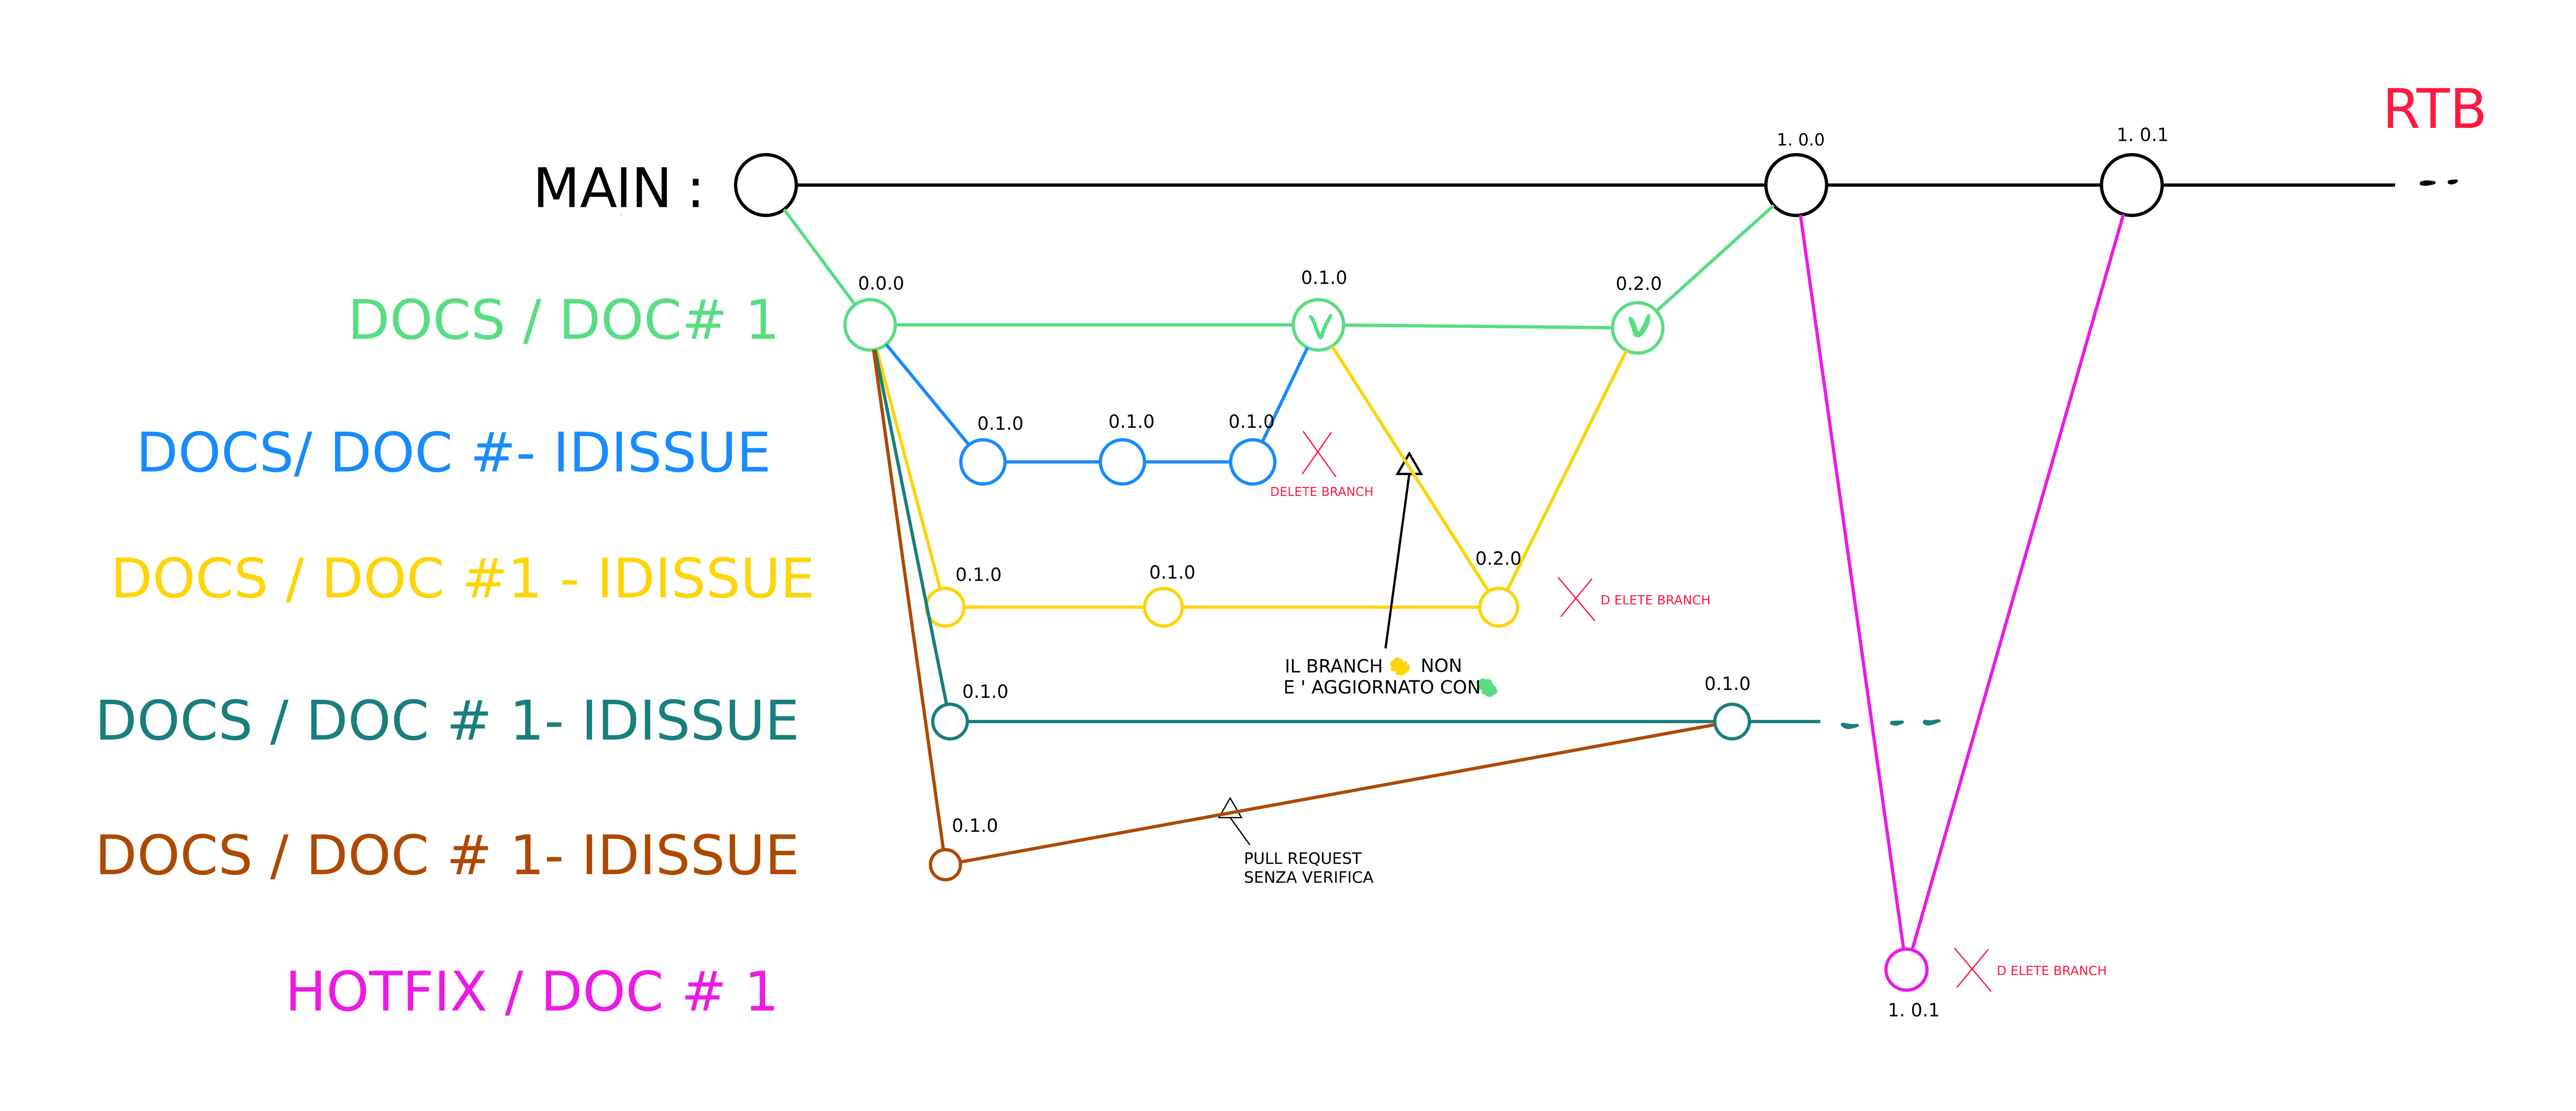
\includegraphics[scale = 0.07]{template/images/workflow.jpg}
        \end{center}

        \subsubsection{Commits}\label{inf:comm}
        E'preferibile che ogni commit abbia una singola responsabilità per cambiamento.
        I commits non possono essere effettuati direttamente sui branch protetti ma per contribuire con delle aggiunte o
        modifiche sarà necessario aprire una Pull Request, motivo per il quale abbiamo introdotto dei branch derivati.
        I messaggi di commit dovranno seguire la seguenti strutture sintattiche:
        \begin{center}
            \textbf{add: [NOME-DOCUMENTO]-[ID-ISSUE]\\
            change: [COSA]\\
            restructure: [COSA]}
        \end{center}
        dove: 
        \begin{itemize}
            \item \textbf{add}: viene utilizzato per il primo un primo commit;
            \item \textbf{change}: per i successivi commit, nei quali si va a modificare il documento già esistente;
            \item \textbf{restructure}: indica una ristrutturazione del branch main per quanto riguarda l'organizzazione delle cartelle e/o la modifica di action o template di issue;
            \item \textbf{NOME-DOCUMENTO}: indica il nome del documento creato;
            \item \textbf{NOME-SEZIONE}: indica la sezione relativa al documento creato;
            \item \textbf{COSA}: breve descrizione di cosa di è aggiunto e/o fatto.
        \end{itemize}

        Notare però che dopo l'approvazione di una Pull Request tutti i commit
        relativi verranno raggruppati in un unico commit, il quale titolo deve rispettare la struttura sintattica descritta in
        seguito.
        \begin{center}
            \textbf{Update: [NOME-DOCUMENTO] to [VERSONE]}
        \end{center}
        dove:

        \begin{itemize}
            \item \textbf{NOME-DOCUMENTO}: indica il nome del documento nel quale sono state verificate le modifiche;
            \item \textbf{VERSIONE}: indica il numero di versione aggiornata.
        \end{itemize}
        Per quanto riguarda il commento facoltativo, si lascia quello di default proposto da GitHub, ovvero un elenco puntato di tutti i commit che verranno raggruppate.\\
        

        Per aggiornare direttamente il main si è deciso di disabilitare temporaneamente
        il protection, eseguire un commit con delle modifiche, con la struttura sintattica elencata sopra, e in fine attivare nuovamente il protection.
        Questa soluzione è stata adottata perché il team ritiene sia più veloce e semplice apportare modifiche a template e action in questo modo
        rispetto che alla creazione di un branch e ad un successivo Pull Request, inoltre il branch main una volta ultimate le automazioni non verrà più modificato se non dai merge
        scatenati delle Pull Request.

        \subsubsection{Pull requests}\label{inf:pr}
        Per effettuare un merge su un branch protetto si deve aprire, da GitHub, una Pull Request. Questa
        permette di verificare il lavoro svolto prima di integrarlo con un branch protetto ed eseguire un veloce test di compilazione della sezione aggiunta.
        Alla creazione di una Pull Request bisogna associare:
        \begin{itemize}
            \item \textbf{Title}: [NOME-DOCUMENTO]-[NOME-SEZIONE];
            \item \textbf{Verificatori in carica}: hanno il compito di trovare eventuali errori o mancanze e fornire un feedback
            riguardante il contenuto direttamente su GitHub attraverso un commento, sulla stessa Pull Request.
            Non sarà possibile effettuare il merge finché tutti i commenti di revisione non saranno stati risolti
            con, al termine, l'approvazione di almeno uno dei verificatori e il test di build non dia esito positivo;
            \item \textbf{Descrizione}: contiene una lista riassuntiva di cio' che è stato fatto includendo le issue completate, e quindi da chiudere,
            con la sintassi
            \begin{center}
                \textbf{\textit{close ID-ISSUE}}
            \end{center}
            in modo tale che vengano tutte chiuse in automatico quando la Pull request verrà accettata;
            \item \textbf{Gli assegnatari}: coloro che hanno anche il compito di apportare le modifiche necessarie al documento;
            \item \textbf{Labels}: che riassumono di che natura è la Pull Request.
        \end{itemize}
        dove:

        \begin{itemize}
            \item \textbf{NOME-DOCUMENTO}: indica il nome del documento sul quale si sta lavorando e richiedendo l'approvazione;
            \item \textbf{NOME-SEZIONE}: indica la sezione relativa al documento creato;
            \item \textbf{ID-ISSUE}: indica il numero identificativo associato alla issue relativa alla modifica del documento.
        \end{itemize}

        Per una descrizione più dettagliata delle issue si faccia riferimento a \nameref{inf:its}

        Per i commit relativi alle Pull Requests seguire le regole descritte nella sezione \nameref{inf:pr}

        \subsubsection{Milestones}
        Esistono 2 tipi di milestone:
        \begin{itemize}
            \item \textbf{Interne}: indicano uno sprint;
            \item \textbf{Esterne}: indicano un traguardo intermedio significativo per il progetto.
        \end{itemize}
        Ad entrambe le milestones possono essere assegnate delle issue per verificarne il raggiungimento e per tenere traccia
        della percentuale di progressione dello sprint.
        Ogni milestone ha una scadenza che viene fissata da tutto il gruppo. Una delle prime milestone esterne create è
        relativa alla \textit{Requirements and Technology Baseline} e di conseguenza la realizzazione di un \textit{PoC}.


        \subsubsection{Project board}
        Viene utilizzata un' unica project board per tracciare tutte le issue della repository, fungendo da backlog del progetto.
        La project board è divisa nelle seguenti sezioni:
        \begin{itemize}
            \item \textbf{Backlog}: issue che non sono ancora state iniziate o assegnate;
            \item \textbf{In progress}: issue che sono state assegnate e a cui almeno un membro, tra gli assegnatari, ha iniziato a lavorarci;
            \item \textbf{Done}: issue terminate e chiuse, con documenti o codice verificati.
        \end{itemize}
        Esempio di workflow potrebbe essere il seguente:
        \begin{enumerate}
            \item Viene creata l'issue ed inserita all'interno della sezione ”Backlog” della project board
            \item Quando viene presa in carico, l'issue viene spostata nella sezione ”In Progress” fino al suo completamento
            \item L'incaricato, una volta risolta, apre una Pull Request a cui assegna la issue, come descritto nella sezione \nameref{inf:pr}.
            \item Dopo l'approvazione della Pull Request la issue verrà chiusa e spostata in modo automatico nella sezione ”Done”.
        \end{enumerate}


        \subsubsection{Issue Tracking System}\label{inf:its}
        Il gruppo utilizza l'issue tracking system di Github per tenere traccia delle issue create. Le issue verranno
        create dall'amministratore, ma la loro assegnazione verrà effettuata dai membri del gruppo in modo autonomo, in base
        alla priorità, ruoli e disponibilità.
        Per marcare le issue secondo criteri di interesse vengono utilizzate delle labels.
        \begin{itemize}
            \item \textbf{P1}: indica una issue o pull request a priorità alta;
            \item \textbf{P2}: indica una issue o pull request a priorità media;
            \item \textbf{P3}: indica una issue o pull request a priorità bassa;
            \item \textbf{bug}: indica una issue o pull request relativa ad un errore/bug nel codice;
            \item \textbf{code}: indica una issue o pull request relativa al codice;
            \item \textbf{documentation}: indica una issue o pull request relativa alla documentazione;
            \item \textbf{enhancement}: indica una issue o pull request relativa al miglioramento di scrittura documentazione o codice;
            \item \textbf{wontfix}: indica una issue che verrà ignorata per motivi di tempo o perché punta ad una azione facoltativa.
        \end{itemize}
        Nel caso un membro del gruppo dovesse rendersi conto che l'issue che sta svolgendo potrebbe essere
        suddivisa in ulteriori issue, dovrà rivolgersi al responsabile per notificarlo di ciò, il quale, se d'accordo,
        darà il compito all'amministratore di modificare/aggiungere delle issue.
        Per rendere la creazione di issue più veloce si sono creati dei template in base al tipo di issue che si vuole inserire, e che richiedono degli input
        specifici.
        \begin{itemize}
            \item  \textbf{TO-DO per documenti}
            \begin{itemize}
                \item \textbf{Titolo} : [NOME-DOCUMENTO]-[NOME-SEZIONE];
                \item \textbf{Oggetto di discussione} (facoltativo): [NOME-VERBALE];
                \item \textbf{Codice verbale}: il codice del \textit{tracciamento delle decisioni} riportato a fine di ogni verbale;
                \item \textbf{Link verbale}: un collegamento ipertestuale al documento per accedervi direttamente;
                \item \textbf{Ruolo}: il ruolo che l'attività puntata della issue richiede;
                \item \textbf{Informazione da implementare}: lista in \textit{Markdown} di tutte le possibili parti della sezione da implementare.
            \end{itemize}
            \item  \textbf{To-DO per codice}
            \begin{itemize}
                \item \textbf{Titolo} : [CODICE-CASO-USO]-[NOME-FEATURES];
                \item \textbf{Oggetto di discussione} (facoltativo): [NOME-VERBALE];
                \item \textbf{Ruolo}: il ruolo che l'attività puntata della issue richiede;
                \item \textbf{Informazione da implementare}: breve descrizione di cosa, la feature aggiunta, deve fare o quali requisiti deve soddisfare.
            \end{itemize}
            \item  \textbf{Bug nel codice}
            \begin{itemize}
                \item \textbf{Titolo}: [CODICE-CASO-USO]-[NOME-FEATURES];
                \item \textbf{Descrizione bug}: breve descrizione del bug;
                \item \textbf{Passi per riprodurlo}: lista numerata in \textit{Markdown} per riassumere i passi da eseguire in modo tale che un'altro programmatore lo possa replicare;
                \item \textbf{Comportamento aspettato}: breve descrizione del comportamento aspettato;
                \item \textbf{Idea sul motivo} (facoltativo): se esiste, una veloce descrizione di un possibile motivo in modo tale da accelerare il processo di debug e correzione.
            \end{itemize}
            \item  \textbf{Correzione della documentazione}
            \begin{itemize}
                \item \textbf{Titolo} : [NOME-DOCUMENTO]-[NOME-SEZIONE];
                \item \textbf{Descrizione}: breve descrizione di cosa correggere nella sezione indicata.
            \end{itemize}
            \item  \textbf{Miglioramento della documentazione}
            \begin{itemize}
                \item \textbf{Titolo} : [NOME-DOCUMENTO]-[NOME-SEZIONE];
                \item \textbf{Descrizione}: breve descrizione di cosa modificare/migliorare e come, nella sezione indicata.
            \end{itemize}
            \item  \textbf{Miglioramento del codice}
            \begin{itemize}
                 \item \textbf{Titolo} : [CODICE-CASO-USO]-[NOME-CASO-USO];
                 \item \textbf{Descrizione}: breve descrizione di cosa modificare/migliorare e come, nella relativa parte di codice indicata.
            \end{itemize}
        \end{itemize}
        dove:

        \begin{itemize}
            \item \textbf{NOME-DOCUMENTO}: indica il nome del documento sul quale si sta lavorando;
            \item \textbf{NOME-VERBALE}: indica il nome del verbale nel quale si è discusso della relativa attività rappresentata successivamente tramite una issue;
            \item \textbf{NOME-SEZIONE}: indica la sezione relativa al documento;
            \item \textbf{CODICE-CASO-USO}: indica il nome del caso d'uso nel quale si sta lavorando;
            \item \textbf{NOME-FEATURES}: indica il nome della feature relativa al caso d'uso.
        \end{itemize}


        \subsubsection{Discord}
        Strumento utilizzato per la comunicazione, in modo sincrono, tra i componenti del gruppo.\\
        Sono creati diversi canali:
        \begin{itemize}
            \item \textbf{Link} : canale testuale per avere dei collegamenti ipertestuali a risorse e riferimenti utili;
            \item \textbf{Utility} : canale testuale per la condivisione di media generici come loghi, disegni illustrativi per determinati workflow e appunti riguardanti le riunioni;
            \item \textbf{General}: canale vocale dedicato alle riunioni interne, al termine delle quali verrà redatto un verbale.
        \end{itemize}

        \subsubsection{Telegram}
        Strumento utilizzato per la comunicazione, in modo asincrono, tra i componenti del gruppo.\\
        Sono creati 2 distinti gruppi:
        \begin{itemize}
            \item \textbf{Generale} : gruppo dedicato alle comunicazioni brevi e poco importanti;
            \item \textbf{Daily Scrum} : gruppo dedicato all' attivita di Daily Scrum, descritto nella sezione \nameref{inf:sprint}.
        \end{itemize}

    \subsection{Gestione dei dubbi e conflitti}
        Nel caso sorgano dubbi, questi verranno risolti, in base all'urgenza, 
        tramite comunicazione nel canale Telegram o durante la riunione interna 
        settimanale. \\
        I conflitti invece verranno prevalentemente discussi in sede di riunione 
        interna, con l'obiettivo di trovare una soluzione condivisa che consenta 
        al progetto di progredire secondo una visione comune.
\pagebreak


\section{Processi di Supporto}
I processi di supporto contribuiscono a rendere i processi primari più efficienti ed efficaci.
    \subsection{Documentazione}
        \subsubsection{Descrizione}
        Questa sezione contiene tutte le norme che ogni membro del gruppo dovrà seguire durante 
        la stesura della documentazione.\\
        Fornisce le indicazioni utili per ottenere una forma uniforme dei documenti e permette di operare seguendo linee guida durante tutte le fasi del ciclo di vita di un documento: creazione, stesura, verifica\textsubscript{g} ed 
        eventuali modifiche, fino ad arrivare all'approvazione\textsubscript{g} e quindi alla pubblicazione del documento.
        \subsubsection{Ciclo di vita di un documento}
        \begin{itemize}
            \item \textbf{Creazione}: viene creato un nuovo branch\textsubscript{g}, che prende il nome del documento stesso, e qui verrà caricato il template, in questo branch\textsubscript{g} ci saranno solamente le versioni verificate del documento;
            \item \textbf{Stesura}: per la stesura verrà creato un sotto-branch\textsubscript{g}, caratterizzato dal numero della issue che richiede la stesura, in seguito si procede con la stesura delle sezioni necessarie, tracciando i cambiamenti nel registro delle modifiche e aggiornando la versione;
            \item \textbf{Verifica\textsubscript{g}}: prima di considerarsi completata, ogni modifica al documento deve essere verificata da un verificatore in carica, tramite una Pull Request\textsubscript{g} viene messo in esame quanto aggiunto al documento rispetto alla versione precedente, si presentano due casi:
            \begin{itemize}
                \item \textbf{Pull Request\textsubscript{g} accettata}: il verificatore non trova errori e considera il lavoro 'verificato', viene accettata la Pull Request\textsubscript{g} e viene fatto il merge tra il branch\textsubscript{g} di lavoro e il branch\textsubscript{g} del documento, viene così chiusa la issue assegnata e chiuso il branch di lavoro;
                \item \textbf{Pull Request\textsubscript{g} rifiutata}: il verificatore non considera la stesura adeguata e procede a segnalare errori ed eventuali correzioni, la Pull Request\textsubscript{g} viene rifiutata e si continua a lavorare nel sotto-branch\textsubscript{g};
            \end{itemize}
            \item \textbf{Approvazione\textsubscript{g}}: Una volta che tutte le sezioni sono state verificate, e il documento è pronto per essere pubblicato, si procede con l'approvazione\textsubscript{g}, effettuata dal responsabile, utilizziamo questa procedura:
            \begin{itemize}
                \item Viene aperta una Pull Request\textsubscript{g} per fare il merge del branch\textsubscript{g} dedicato al documento con il main;
                \item Il responsabile rilegge ed analizza il documento nella sua interezza, se riscontra errori o problematiche, rifiuta la Pull Request\textsubscript{g}, segnala ai verificatori le modifiche necessarie e si procede come descritto sopra;
                \item Nel caso andasse tutto bene, il responsabile aggiorna il registro delle modifiche aggiungendo una riga con la versione di pubblicazione, e contrassegna il documento come 'Approvato';
                \item Il documento viene quindi pubblicato nel ramo main, e reso disponibile pubblicamente.
            \end{itemize}
        \end{itemize}
        Solo alla pubblicazione nel ramo main il documento verrà compilato e reso disponibile in formato '.pdf'.
        \newpage
        \subsubsection{Struttura}
        Ogni documento è caratterizzato da un template, che presenta queste caratteristiche:
        \begin{itemize}
            \item \textbf{Intestazione}: la prima pagina di ogni documento, contiene:
            \begin{itemize}
                \item Logo del gruppo;
                \item Indirizzo email del gruppo;
                \item Titolo del documento;
                \item Informazioni sul documento, che comprendono:
                \begin{itemize}
                    \item Versione;
                    \item Stato: in redazione oppure approvato;
                    \item Uso: interno o esterno;
                    \item Approvazione\textsubscript{g}: indica il nome dell'elemento del gruppo che ha approvato il documento;
                    \item Redazione: indica il nome o i nomi di chi si è occupato della stesura;
                    \item Verifica\textsubscript{g}: indica il nome del verificatore o dei verificatori;
                    \item Distribuzione: elenco delle persone o organizzazioni a cui è destinato il documento.
                \end{itemize}
                \item Descrizione: una breve descrizione di cosa contiene il documento;
            \end{itemize}
            \item \textbf{Registro delle modifiche}: contiene la tabella dove verranno registrati i cambiamenti e le versioni che un documento attraversa prima di giungere alla versione finale, include le seguenti colonne:
            \begin{itemize}
                \item Versione;
                \item Data;
                \item Autore;
                \item Descrizione: una descrizione riassuntiva di ciò che è stato aggiunto o modificato;
                \item Verificatore.
            \end{itemize}
            \item \textbf{Indice}: elenco ordinato dei titoli dei capitoli, per facilitare la navigazione;
            \item \textbf{Contenuto}: varia a seconda del documento.
        \end{itemize}
        % + tutte le convenzioni
        \subsubsection{Convenzioni}
        Al fine di ottenere una stesura della documentazione omogenea, e quindi più professionale, verranno seguite queste convenzioni:
        \paragraph{Date}
        Per garantire un ordinamento in ordine cronologico in fase di pubblicazione, dal più recente al meno recente, verrà utilizzato il formato \textbf{yyyy-mm-dd} nel caso la data debba essere indicata nel nome del documento (vale per verbali interni/esterni), 
        per indicare una data all'interno del documento, verrà utilizzato il formato \textbf{dd-mm-yyyy}.
        \paragraph{Nomi di persona} 
        All'interno dei documenti i nomi di persona saranno rappresentati da cognome e nome.
        \paragraph{Elenchi puntati}
        Gli elenchi puntati saranno gestiti in questo modo:
        \begin{itemize}
            \item Ogni elemento dell'elenco deve iniziare con la lettera maiuscola;
            \item Ogni elemento dell'elenco deve terminare con ';', ad eccezione dell'ultimo che terminerà con '.';
            \item Dopo i due punti la prima parola deve iniziare con la lettera minuscola.
        \end{itemize}
        \paragraph{Stile del testo}
        \begin{itemize}
            \item \textbf{Grassetto}: utilizzato per i titoli delle sezioni, per i sottotitoli, per i paragrafi e per parole tecniche o termini specifici che necessitano di evidenza nel contesto;
            \item \textbf{Corsivo}: utilizzato quando vengono scritti nomi di documenti, nome del gruppo o indirizzo email del gruppo.
        \end{itemize}
        \paragraph{Link}
        All'interno dei documenti i link saranno strutturati in questo modo:
        \begin{itemize}
            \item Breve descrizione della destinazione del link: \textbackslash url\{indirizzo\_del\_link\}.
        \end{itemize}
        \paragraph{Terminologia inglese}    
        Tutti i termini in lingua inglese saranno riportati al singolare, in quanto questa scelta risulta più coerente con l'uso comune e l'assonanza nella lingua italiana. Ad esempio, termini come "file" o "commit" verranno sempre utilizzati nella loro forma singolare, anche quando si riferiscono a concetti plurali, per evitare ambiguità o traduzioni non naturali.\\
        Per quanto riguarda il genere (maschile o femminile), verrà specificato all'interno del \textit{glossario}, così da uniformare l'interpretazione e garantire chiarezza, specialmente nei casi in cui il termine inglese non abbia un corrispettivo diretto o il genere non sia immediatamente evidente. Questa scelta mira a favorire una lettura fluida e una comprensione condivisa del testo.
        \paragraph{Acronimi} 
        Tutti gli acronimi seguiranno queste regole:
        \begin{itemize}
            \item L'acronimo deve essere scritto in maiuscolo;
            \item L'articolo davanti a un acronimo deve concordare in genere e numero con il termine principale che l'acronimo rappresenta. Nel caso di acronimi derivati da termini stranieri, la concordanza va basata sul significato tradotto o percepito in italiano. Questo garantisce una corretta integrazione dell'acronimo nella struttura grammaticale della lingua;
            \item Ogni acronimo deve essere inserito nel glossario, accompagnato da una spiegazione dettagliata del suo significato, per garantire chiarezza e comprensione.
        \end{itemize}
        \subsubsection{Strumenti per la stesura}
        Per la stesura dei documenti verrà usato il linguaggio Latex, un linguaggio di marcatura per la preparazione di testi, basato sul programma di
        composizione tipografica TEX, tutta la documentazione prodotta è contenuta nella cartella 'Docs'. I documenti seguono una struttura comune:
        \begin{itemize}
            \item Cartella 'config' contenente il file 'changelog\_input' che permette di compilare i campi della tabella di registrazione delle modifiche;
            \item Cartella 'template' contenente:
            \begin{itemize}
                \item File 'changelog': questo file contiene la definizione di un comando chiamato \texttt{\char`\\changelogTable}, che serve per generare la tabella formattata;
                \item File 'package': configura pacchetti e comandi per personalizzare l'impaginazione, le tabelle, le intestazioni, la numerazione e la formattazione di testo, inclusi glossari e codici;
                \item Cartella 'Images' contenente le immagini inserite nel documento.
            \end{itemize}
            \item File 'main' include i file e i pacchetti necessari a comporre il file;
            \item File 'titlepage' contenente il template della pagina di intestazione.
        \end{itemize}
        Oltre a questi files, verrà creato un file per ogni sezione, per garantire maggiore ordine all'organizzazione del documento, e facilitare la suddivisione dei compiti.
        \subsubsection{Documentazione interna}
        La documentazione interna è composta da tutti i documenti che contengono informazioni utili per il gruppo,  
        ma saranno comunque resi pubblici all'interno del repository, e nella schermata creata tramite GitHub Pages\textsubscript{g}.\\
        La documentazione interna è composta da:
        \begin{itemize}
            \item \textit{\textbf{Verbali Interni}}: hanno lo scopo di riportare ciò che viene detto e discusso durante la riunione interna, ossia tra i soli membri del gruppo, 
            rispetta la struttura generale dei documenti e le convenzioni, il nome del file deve avere la forma 'VI\_yyyy-mm-dd', per garantire l'ordinamento.
            \\Nei \textit{verbali interni} la struttura del contenuto assume questa forma:
            \begin{itemize}
                \item \textbf{Informazioni generali}: contiene informazioni circa i dettagli sull'incontro, nello specifico:
                \begin{itemize}
                    \item Luogo;
                    \item Data;
                    \item Ora di inizio;
                    \item Ora di fine;
                    \item Partecipanti.
                \end{itemize}
                \item \textbf{Motivo della riunione}: breve descrizione narrativa di cosa è stato trattato in quell'incontro, descrive i motivi per cui è stata fatta la riunione;
                \item \textbf{Resoconto}: descrive i temi trattati nel dettaglio, partendo dal motivo per il quale sono stati sollevati e arrivando alla decisione presa dal gruppo a seguito di una discussione;
                \item \textbf{Prossimi obiettivi}: elenco puntato che descrive gli obiettivi che il gruppo si impegna a portare a termine nel breve periodo, indicativamente prima della riunione successiva;
                \item \textbf{Tracciamento delle decisioni}: tabella che riassume le decisioni prese in quella riunione indicandone:
                \begin{itemize}
                    \item \textbf{Codice}: in formato VI Y.Z, dove Y indica il numero del \textit{verbale} (incrementale rispetto agli altri), Z indica il numero dell'argomento trattato (non per importanza, ma per ordine di discussione);
                    \item \textbf{Descrizione}: descrizione in poche parole dell'argomento trattato.
                \end{itemize} 
                \end{itemize}
        \item \textit{\textbf{Studio di fattibilità}}: documento interno di valutazione dei capitolati proposti dalle aziende per il progetto didattico, con lo scopo di selezionare il progetto migliore a cui candidarsi secondo valutazioni 
        prese da parte del gruppo.\\
        Il documento, per ogni capitolato, espone una breve descrizione del prodotto che l'azienda chiede di sviluppare, seguito da una serie di pro e contro emersi in base a criteri soggettivi dei membri del gruppo.
        \\La valutazione è fatta sulla base di:
        \begin{itemize}
            \item \textbf{Presentazione del capitolato}: una presentazione più curata e dettagliata riscontra maggiore successo in fase di valutazione;
            \item \textbf{Interesse del gruppo al tema del progetto}: un capitolato porta con se un tema, viene valutato quanto ogni capitolato sia interessante, per apportare un impatto positivo allo svolgimento da parte del gruppo;
            \item \textbf{Tecnologie da utilizzare}: il contesto tecnologico di comune interesse porta maggiore produttività ed entusiasmo all'interno del gruppo;
            \item \textbf{Conoscenze pregresse}: un capitolato può risultare più o meno complicato da svolgere a seconda delle conoscenze acquisite nel percorso dai membri del gruppo;
            \item \textbf{Supporto da parte dell'azienda}: maggiore è il supporto offerto dall'azienda, migliore sarà la valutazione del capitolato.
        \end{itemize}  
        Il documento offre una panoramica completa di tutti i capitolati, potendoli valutare minuziosamente prima di esprimere una valutazione.
        \item \textit{\textbf{Norme di progetto}}: documento interno che contiene le norme applicate dai membri del gruppo durante il ciclo di vita del prodotto, rispetta la struttura generale della documentazione, il corpo di questo documento è composto da:
        \begin{itemize}
            \item \textbf{Introduzione}: contiene una breve descrizione dello scopo del documento e del contesto in cui viene applicato;    
            \item \textbf{Processi primari}: definizione dei processi primari, nel nostro caso:
            \begin{itemize}
                \item Fornitura: definizione e regole di fornitura e rapporto con il proponente;
                \item Sviluppo: definizione e regole di sviluppo per quanto riguarda l'analisi dei requisiti, la progettazione e la codifica.
            \end{itemize}
            \item \textbf{Processi organizzativi}: costituisce la definizione dei processi per quanto riguarda l'organizzazione del gruppo, in termini di:
            \begin{itemize}
                \item Pianificazione: viene definito il metodo di lavoro, i ruoli che verranno assegnati e le responsabilità che da essi ne derivano;
                \item Modalità di comunicazione: vengono definite le modalità attraverso le quali il gruppo comunicherà internamente ed esternamente (qualsiasi comunicazione che comprenda un soggetto esterno al gruppo di lavoro);
                \item Modalità di riunione: vengono definite le modalità con le quali si svolgeranno le riunioni, interne ed esterne;
                \item Gestione di infrastrutture: descrizione delle infrastrutture utilizzate per lo sviluppo del progetto, affinchè venga garantita affidabilità e sicurezza;
                \item Gestione dei dubbi o conflitti.
            \end{itemize}

            \item \textbf{Processi di supporto}: definizione dei processi di supporto, nel nostro caso:
            \begin{itemize}
                \item Documentazione: descrive le regole e la struttura dei documenti, il ciclo di vita e le convenzioni da utilizzare durante la stesura. Vengono descritti i documenti presenti nel repository.
                \item Gestione della configurazione: descrive come gestire il versionamento dei documenti.
                \item Accertamento della qualità: descrive come vengono verificati i documenti;
                \item Validazione: comprende le regole e la definizione di validazione.
            \end{itemize}
            \item \textbf{Standard di qualità ISO/IEC 9126}: descrizione dello standard da cui il gruppo estrarrà le norme per la misurazione della qualità del software;
            \item \textbf{Standard di qualità ISO/IEC 12207:1995}: descrizione dello standard scelto per garantire la qualità dei processi relativi al ciclo di vita del software;
            \item \textbf{Metriche}: sezione del documento in cui verranno riportate e descritte tutte le metriche adottate per la valutazione qualitativa dei processi e dei prodotti, verrà spiegato in dettaglio il significato di ogni metrica e il modo in cui le valutazioni verranno calcolate, spiegando i procedimenti.
             
        \end{itemize}
        \end{itemize}
        \subsubsection{Documentazione esterna}
        La documentazione esterna è composta da tutti i documenti che interessano anche al proponente e al committente.
        \begin{itemize}
            \item \textit{\textbf{Verbali esterni}}: verbali frutto di incontri fra i membri del gruppo e soggetti esterni ad esso.\\
            Seguono la struttura dei verbali interni, il nome del file deve avere la forma 'VE\_yyyy-mm-dd', cambia il processo di approvazione\textsubscript{g} del documento, che oltre ad essere approvato internamente, viene approvato esternamente dal soggetto esterno con il quale 
            si è svolto l'incontro, questo per rendere il documento più professionale e garantire coerenza tra il gruppo e il soggetto esterno.
            \item \textit{\textbf{Lettera di candidatura}}: la \textit{Lettera di candidatura} serve per esprimere la volontà di candidarsi allo svolgimento del capitolato scelto dopo aver discusso e redatto lo \textit{Studio di fattibilità}, 
            è composta da:
            \begin{itemize}
                \item Pagina iniziale: viene dichiarato il capitolato per il quale il gruppo ha deciso di candidarsi, elencando i capitolati che più hanno riscontrato interesse da parte del gruppo, 
                inoltre espone una descrizione di cosa aspettarsi dal contenuto del documento;
                \item Resoconto degli incontri: una breve descrizione degli incontri svolti con le aziende riguardo i capitolati elencati nella pagina iniziale;
                \item Motivazione della scelta: espone il motivo per il quale il gruppo ha scelto il capitolato a cui candidarsi.
            \end{itemize}
            \item \textit{\textbf{Diario di bordo}}: documento informale ad uso esterno che permette di interagire settimanalmente con il committente per riportare aggiornamenti sullo stato di avanzamento del progetto, descrivendo tutto ciò che è stato fatto rispetto al \textit{diario di bordo} precedente, 
            e quello che il gruppo si impegna a fare nel periodo successivo, vengono inoltre riportati dubbi e domande da porre al committente.
            Vengono elaborati tramite la piattaforma online 'Canva.com', che permette di creare presentazioni collaborative, accessibili online.\\ 
            La struttura del \textit{diario di bordo} è composta da 4 slides contenenti:
            \begin{itemize}
                \item \textbf{Slide 1}: slide di presentazione che contiene:
                \begin{itemize}
                    \item Logo;
                    \item Nome del gruppo;
                    \item Indirizzo email del guppo;
                    \item Titolo del documento: il titolo del \textit{diario di bordo} segue una sintassi prefissata ovvero 'Diario di bordo \#N', dove N è un numero che incrementa ad ogni presentazione.
                \end{itemize}
                \item \textbf{Slide 2}: contiene ciò che è stato svolto nel periodo trascorso;
                \item \textbf{Slide 3}: contiene ciò che il gruppo si impegna a portare a termine nel periodo successivo;
                \item \textbf{Slide 4}: contiene dubbi da chiarire e difficoltà incontrate dal gruppo.
            \end{itemize}
            \item \textit{\textbf{Piano di progetto}}: il documento \textit{piano di progetto} ha lo scopo di supportare la gestione delle risorse per quanto riguarda l'avanzamento del progetto, per riuscire a portarlo a termine entro la data decisa.\\
            Il \textit{piano di progetto} ha inoltre la funzione di descrivere il modello di sviluppo adottato, e di monitorarlo tramite la suddivisione in periodi, per analizzare il lavoro svolto e poter apportare miglioramenti con il passare del tempo.
            \\La struttura del documento segue la struttura generale, per quanto riguarda il corpo, è composto da queste sezioni:
            \begin{itemize}
                \item \textbf{Introduzione}: breve introduzione che descrive cosa aspettarsi dal contenuto del documento, sezione composta da:
                \begin{itemize}
                    \item Scopo del documento;
                    \item Scopo del prodotto;
                    \item Riferimenti normativi e informativi.
                \end{itemize}
                \item \textbf{Analisi dei rischi}: sezione che riassume i rischi a cui il gruppo si espone a seguito dell'aggiudicazione del capitolato, suddivisi in:
                \begin{itemize}
                    \item Rischi riguardanti i requisiti;
                    \item Rischi tecnologici;
                    \item Rischi organizzativi;
                    \item Rischi personali.
                \end{itemize}
                \item \textbf{Modello di sviluppo}: sezione che descrive il modello di sviluppo adottato dal gruppo, che si basa su un approccio agile. Viene fornita una descrizione completa del modello, illustrandone i principi fondamentali, le metodologie applicate e le motivazioni che hanno portato alla scelta di questo approccio;
                \item \textbf{Pianificazione}: sezione che descrive lo svolgimento delle attività suddiviso per periodi, fornendo un riassunto degli obiettivi previsti per ciascuno Sprint. Verranno indicati i risultati che il gruppo intende raggiungere e sarà incluso un diagramma di Gantt per visualizzare la pianificazione delle tempistiche e il progresso delle attività;
                \item \textbf{Preventivo}: sezione in cui viene pianificata in dettaglio la suddivisione dei ruoli con le corrispondenti ore di lavoro, per fornire un preventivo rispetto al periodo a cui ci si sta accingendo;
                \item \textbf{Consuntivo}: sezione che presenta i dati raccolti al termine di ciascun periodo, confrontandoli con le previsioni indicate nella sezione di preventivo. Verranno riportate le ore effettive di lavoro svolte e il relativo costo, accompagnati da un resoconto dettagliato che confronta le stime iniziali con i valori effettivi. Questo confronto permette di valutare eventuali scostamenti e di analizzarne le cause;
                \item \textbf{Attualizzazione dei rischi}: sezione dove vengono riportati i rischi che si sono verificati durante lo svolgimento del progetto e le relative misure di mitigazione attuate.
            \end{itemize}

            \item \textit{\textbf{Piano di qualifica}}: il documento \textit{piano di qualifica} descrive i principi guida e le attività messe in atto dal team per assicurare che i processi adottati e prodotti sviluppati durante lo svolgimento del progetto siano di alta qualità per quanto riguarda le misure di efficienza ed efficacia.\\
            In questo documento verranno presentati i risultati delle analisi quantitative condotte per valutare le performance del team, evidenziando eventuali criticità e azioni correttive intraprese.
            \\La struttura del documento segue la struttura generale. Per quanto riguarda il corpo, è composto da queste sezioni:
            \begin{itemize}
                \item \textbf{Introduzione}: breve introduzione che descrive cosa aspettarsi dal contenuto del documento, riporta lo scopo del documento, lo scopo del prodotto, i riferimenti normativi e informativi;
                \item \textbf{Qualità di processo}: viene indicato lo standard adottato per la valutazione dei processi e quello per garantire un miglioramento continuo.\\
                                                    Seguono poi quattro sezioni:
                                                    \begin{itemize}
                                                        \item \textbf{Processi primari}: riporta una descrizione dei processi di fornitura e di sviluppo, e specifica le metriche per l'accertamento della qualità;
                                                        \item \textbf{Processi di supporto}: riporta una descrizione dei processi di documentazione, accertamento della qualità e verifica, specificando per ogni processo le metriche utilizzate; 
                                                        \item \textbf{Processi organizzativi}: riporta una descrizione del processo di gestione di progetto e specifica le metriche da adottare per garantirne la qualità;
                                                        \item \textbf{Metriche}: contiene una tabella con le metriche adottate per la valutazione della qualità di processo, riportandone:
                                                        \begin{itemize}
                                                            \item \textbf{Codice identificativo}: costituito da MPC[N], dove N rappresenta il numero della metrica di riferimento;
                                                            \item \textbf{Nome}: nome della metrica;
                                                            \item \textbf{Valore accettabile}: valore minimo accettabile per la metrica;
                                                            \item \textbf{Valore ottimale}: valore ottimo per la metrica.
                                                        \end{itemize}
                                                    \end{itemize}
                                                    \item \textbf{Qualità di prodotto}: viene indicato lo standard di riferimento adottato dal team per garantire la qualità del software e della documentazione prodotta.
                                                    \begin{itemize}
                                                        \item \textbf{Documenti}: riporta una descrizione dei parametri su cui si basa la valutazione della documentazione prodotta, ovvero comprensibilità e correttezza, e si riportano le metriche di riferimento;
                                                        \item \textbf{Software}: fornisce una descrizione degli obiettivi prefissati dal team per garantire la qualità nella produzione del software, focalizzandosi sui seguenti aspetti:
                                                        \begin{itemize}
                                                            \item Funzionalità;
                                                            \item Affidabilità;
                                                            \item Usabilità;
                                                            \item Efficienza;
                                                            \item Manutenibilità;
                                                            \item Portabilità.
                                                        \end{itemize}
                                                        Fornendone una descrizione e riportando le metriche di riferimento.
                                                        \item \textbf{Metriche}: contiene una tabella con le metriche adottate per la valutazione della qualità di prodotto, riportandone:
                                                        \begin{itemize}
                                                            \item \textbf{Codice identificativo}: costituito da MPD[N], dove N rappresenta il numero della metrica di riferimento;
                                                            \item \textbf{Nome}: nome della metrica;
                                                            \item \textbf{Valore accettabile}: valore minimo accettabile per la metrica;
                                                            \item \textbf{Valore ottimale}: valore ottimo per la metrica.
                                                        \end{itemize}
                                                    \end{itemize}
            \end{itemize}
            \item \textit{\textbf{Glossario}}: documento che contiene il significato dei termini chiave utilizzati nel progetto (indicati con il pedice 'g'), organizzati in ordine alfabetico, utile per garantire una comprensione comune fornendo spiegazioni concise e precise.
            \\La struttura del \textit{glossario} è composta da sezioni caratterizzate dalle lettere dell'alfabeto in ordine alfabetico, contenenti le parole che hanno come iniziale quella lettera.
        \end{itemize}

    \subsection{Gestione delle configurazione}
        \subsubsection{Scopo}
        La gestione della configurazione è un processo che mira a gestire e controllare i cambiamenti apportati
        a un prodotto software o a un sistema durante il suo ciclo di vita. La gestione della configurazione per
        la documentazione descrive come vengono identificate, controllate, tracciate e gestite le versioni di un
        documento.
        \subsubsection{Versionamento}
        Ogni versione del documento è identificata da un codice di versione nel formato \textbf{Z.Y.X} dove:
        \begin{itemize}
            \item \textbf{Z}: il documento è pronto per una delle revisioni, ovvero tutte le modifiche precedenti sono state approvate dal responsabile;
            \item \textbf{Y}: la sezione aggiunta o modificata di un documento è stata verificata;
            \item \textbf{X}: è stata corretta velocemente qualche incoerenza o errore minore.
        \end{itemize}

    \subsection{Accertamento della qualità}
    \subsubsection{Scopo}
    Lo scopo del processo di accertamento della qualità è di verificare che non siano stati commessi errori nello svolgimento delle attività prefissate, e di garantire il rispetto dei requisiti di qualità descritti nel \textit{piano di qualifica}.
    \subsubsection{Descrizione}
    Il processo di accertamento della qualità viene applicato costantemente sia durante la stesura della documentazione, che durante lo sviluppo del software, il team si impegna a svolgere ogni attività perseguendo gli obiettivi qualitativi discussi e concordati per il soddisfacimento delle metriche adottate e riportate nel \textit{piano di qualifica}.    

    \subsection{Verifica\textsubscript{g}}
        \subsubsection{Scopo}
        Lo scopo del processo di verifica\textsubscript{g} è quello di accertare che non siano stati commessi errori nello svolgimento
        delle attività prefissate. Questo processo viene applicato costantemente sia durante la stesura
        della documentazione, che durante lo sviluppo del software.
        \subsubsection{Descrizione}
        La verifica verrà fatta in maniera efficace adottando questi metodi:
        \begin{itemize}
            \item \textbf{Analisi statica}: non richiede esecuzione dell'oggetto di verifica, quindi applicabile a documentazione e codice, usata per accertare conformità e regole nonché assenza di difetti, adotteremo i due seguenti metodi di lettura:
             \begin{itemize}
                \item \textbf{Walkthrough}: processo in cui il team esamina documenti o codice, in modo strutturato ma informale. L'obiettivo è identificare errori, migliorare la qualità e favorire la comprensione;
                \item \textbf{Inspection}: processo di revisione più formale, in cui i veroficatori controllano documenti o codice per trovare errori e migliorare la qualità eseguendo una lettura mirata dell'oggetto di verifica. Segue regole precise e prevede momenti organizzati, come pianificazione, definizione lista di controllo, lettura e correzione dei difetti.
             \end{itemize}
             \item \textbf{Analisi dinamica}: richiede esecuzione dell'oggetto di verifica, quindi applicabile solo al codice, usata per accertare che il codice sia corretto, non introduca errori nel sistema e soddisfi i requisiti preposti.
        \end{itemize}
        \subsubsection{Verifica\textsubscript{g} della documentazione}
        Al momento della necessità di modificare o aggiungere qualcosa a una sezione di un documento, si procederà in questo modo:
        \begin{enumerate}
            \item Verrà creata una issue che specifica l'attività di modifica o aggiunta da svolgere;
            \item Verrà creato un sotto-branch\textsubscript{g} chiamato 'docs/\textit{nome\_del\_documento}-N' dove con N si intende il numero della issue di riferimento;
            \item Rimanendo in questo sotto-branch\textsubscript{g}, verrà aggiornato il documento;
            \item Una volta terminato, per iniziare il processo di verifica\textsubscript{g} verrà aperta una Pull Request\textsubscript{g};
            \item Uno tra i verificatori in carica durante quello sprint si assegnerà la verifica del documento e modificherà il registro delle modifiche compilando il campo 'Verificatore';
            \item Se la Pull Request\textsubscript{g} avrà esito positivo, ci sarà il merge tra il sotto-branch\textsubscript{g} e il branch\textsubscript{g} principale del documento, con conseguente chiusura della issue e del sotto-branch;
            \item In caso di esito negativo, verranno segnalati gli errori da parte del verificatore tramite commenti, e il redattore si occuperà di risolverli continuando a lavorare nel sotto-branch\textsubscript{g}, fino ad avere il documento verificato.
        \end{enumerate}

        \subsubsection{Verifica\textsubscript{g} del codice}
        Il processo di verifica del codice si attua principalmente attraverso lo sviluppo e l'esecuzione di test, che permettono di eseguire un'analisi dinamica del software, ossia un'analisi che si concentra sul comportamento del programma durante l'esecuzione. I test vengono progettati per garantire che il codice funzioni correttamente in vari scenari e che rispetti i requisiti prefissati. I principali tipi di test utilizzati in questo processo sono:
        \begin{itemize}
            \item \textbf{Test di unità}: verificano il corretto funzionamento delle singole unità o funzioni del codice, testando piccoli blocchi di logica isolati. Questi test sono fondamentali per individuare errori precoci e garantire che ogni componente funzioni come previsto. Vengono scritti dal programmatore che implementa il modulo;
            \item \textbf{Test di integrazione}: verificano che i vari moduli o componenti del sistema interagiscano correttamente tra loro. Questi test sono particolarmente utili per identificare problemi che si verificano quando le diverse parti del sistema vengono messe insieme;
            \item \textbf{Test di regressione}: vengono eseguiti per verificare che le modifiche recenti al codice non abbiano introdotto nuovi errori o causato il malfunzionamento di funzionalità precedentemente funzionanti. Questi test sono essenziali per mantenere l'integrità del software durante lo sviluppo continuo;
            \item \textbf{Test di sistema}: testano il comportamento complessivo dell'applicazione in un ambiente che simula il più possibile l'ambiente di produzione. Questi test verificano che l'intero sistema funzioni come previsto sotto condizioni realistiche e che tutte le componenti siano correttamente integrate.
        \end{itemize}   
        I test vengono identificati attraverso un codice con questa struttura:
        \textbf{
            \[
            T[\text{Tipo}][ \text{N}]
            \]
            }
        \\Dove N è il codice del test ed è un valore univoco e il tipo può essere:
        \begin{itemize}
            \item \textbf{U}: test di unità;
            \item \textbf{I}: test di integrazione;
            \item \textbf{R}: test di regressione;
            \item \textbf{S}: test di sistema.  
        \end{itemize}
    \subsection{Validazione}
        \subsubsection{Scopo}
        Per la documentazione la validazione corrisponde alla pubblicazione del documento nel branch\textsubscript{g} main.\\
        Questo processo avviene dopo l'ultima verifica\textsubscript{g} e sarà il responsabile a stabilire se il prodotto è accettabile o ha bisogno di
        ulteriori verifiche.

\pagebreak

\section{Standard per la qualità}

\subsection{ISO/IEC 12207:1995}
Per definire, misurare e valutare i processi da attuare nello svolgimento
del progetto, il gruppo adotta lo standard ISO/IEC 12207:1995, che
definisce un modello per i processi di ciclo di vita del software. 
Tale modello suddivide i processi in primari, di supporto e organizzativi.
Ogni processo consiste di più attività, e ogni attività è a sua volta
composta da più task.

\subsubsection{Processi primari}
I processi primari vengono impiegati dalle parti primarie durante il ciclo di 
vita del software. Una parte è detta primaria se avvia o si occupa dello 
sviluppo, dell'operatività o della manutenzione di prodotti software. 
Queste parti sono l'acquirente, il fornitore, lo sviluppatore, l'operatore e il manutentore.

\subsubsubsection{Acquisizione}
Processo che contiene le attività dell'acquirente, ossia l'organizzazione che
acquista un prodotto o servizio software.
\begin{itemize}
    \item Avviamento;
    \item Preparazione della richiesta di proposta;
    \item Preparazione e aggiornamento del contratto;
    \item Controllo dei fornitori;
    \item Accettazione e completamento.
\end{itemize}

\subsubsubsection{Fornitura}
Processo che contiene le attività del fornitore, ossia l'organizzazione che
fornisce il prodotto o servizio software all'acquirente.
\begin{itemize}
    \item Avviamento;
    \item Preparazione della risposta;
    \item Contratto;
    \item Pianificazione;
    \item Esecuzione e controllo;
    \item Revisione e valutazione;
    \item Consegna e completamento.
\end{itemize}

\subsubsubsection{Sviluppo}
Processo che contiene le attività dello sviluppatore, ossia l'organizzazione che
definisce, progetta e implementa il prodotto software.
\begin{itemize}
    \item Implementazione dei processi;
    \item Analisi dei requisiti di sistema;
    \item Progettazione dell'architettura di sistema;
    \item Analisi dei requisiti software;
    \item Progettazione dell'architettura software;
    \item Progettazione dettagliata del software;
    \item Codifica e test del software;
    \item Integrazione software;
    \item Integrazione di sistema;
    \item Installazione del software;
    \item Supporto all'accettazione del software.
\end{itemize}

\subsubsubsection{Processo operativo}
Processo che contiene le attività dell'operatore, ossia l'organizzazione che
fornisce il servizio di gestione del sistema informatico nel suo ambiente 
operativo per i suoi utenti.
\begin{itemize}
    \item Implementazione dei processi;
    \item Test operativo;
    \item Operazioni di sistema;
    \item Supporto utente.
\end{itemize}

\subsubsubsection{Manutenzione}
Processo che contiene le attività del manutentore, ossia l'organizzazione che
fornisce il servizio di manutenzione del prodotto software. Gestisce quindi 
le modifiche al prodotto software per mantenerlo aggiornato e in condizioni operative. 
\begin{itemize}
    \item Implementazione dei processi;
    \item Analisi dei problemi e delle modifiche;
    \item Implementazione delle modifiche;
    \item Revisione/accettazione delle manutenzione;
    \item Migrazione;
    \item Ritiro del software.
\end{itemize}

\subsubsection{Processi di supporto}
Un processo di supporto sostiene un altro processo come parte integrante 
con uno scopo distinto, e contribuisce al successo e alla qualità del progetto software. 
Un processo di supporto è impiegato ed eseguito, se necessario, da un altro processo. 

\subsubsubsection{Documentazione}
Processo per registrare le informazioni prodotte da un'attività o
da un processo di ciclo di vita.
\begin{itemize}
    \item Implementazione del processo;
    \item Progettazione e sviluppo;
    \item Produzione;
    \item Manutenzione.
\end{itemize}

\subsubsubsection{Gestione della configurazione}
Processo che consiste nell'applicare procedure amministrative e tecniche
attraverso il ciclo di vita del software allo scopo di identificare e definire
gli item in un sistema; controllare modifiche e rilasci degli item;
registrare lo stato degli item e le richieste di modifica; assicurare la completezza,
la consistenza e la correttezza degli item.
\begin{itemize}
    \item Implementazione del processo;
    \item Identificazione della configurazione;
    \item Controllo della configurazione;
    \item Resoconto dello stato della configurazione;
    \item Valutazione della configurazione;
    \item Gestione dei rilasci e delle consegne.
\end{itemize}

\subsubsubsection{Accertamento della qualità}
Processi per fornire adeguate garanzie che i processi e i prodotti
siano conformi ai requisiti e aderiscano ai piani stabiliti.
L'accertamento della qualità può utilizzare i risultati di altri
processi di supporto, come la verifica e la validazione.
\begin{itemize}
    \item Implementazione del processo;
    \item Accertamento dei prodotti;
    \item Accertamento dei processi;
    \item Accertamento dei sistemi di qualità.
\end{itemize}

\subsubsubsection{Verifica}
Processo per determinare se i prodotti di una data attività soddisfano
i requisiti e le condizione ad essi imposti nelle precedenti attività.
\begin{itemize}
    \item Implementazione del processo;
    \item Verifica.
\end{itemize}

\subsubsubsection{Validazione}
Processo per determinare se i requisiti e il sistema software
prodotto soddisfano la specifica destinazione d'uso.
\begin{itemize}
    \item Implementazione del processo;
    \item Validazione.
\end{itemize}

\subsubsubsection{Revisione congiunta}
Processo per valutare lo stato e i prodotti di un'attività, ove opportuno.
Le revisioni congiunte avvengono sia a livello di gestione di progetto che
a livello tecnico.
\begin{itemize}
    \item Implementazione del processo;
    \item Revisione della gestione di progetto;
    \item Revisione tecnica.
\end{itemize}

\subsubsubsection{Audit}
Processo per determinare la conformità con i requisiti, i piani 
e il contratto, ove opportuno.
\begin{itemize}
    \item Implementazione del processo;
    \item Audit.
\end{itemize}

\subsubsubsection{Risoluzione dei problemi}
Processo per analizzare e risolvere i problemi (incluse non conformità),
che si presentano durante l'esecuzione di altri processi. 
\begin{itemize}
    \item Implementazione del processo;
    \item Risoluzione dei problemi.
\end{itemize}

\subsubsection{Processi organizzativi}
I processi organizzativi vengono impiegati da un'organizzazione per stabilire 
e attuare una struttura di base costituita dai processi e dal personale,
e per migliorare costantemente tale struttura.

\subsubsubsection{Gestione organizzativa}
Processo che contiene le attività generiche che possono 
essere impiegate da qualunque parte che deve gestire i propri processi.
\begin{itemize}
    \item Avviamento e definizione dello scopo;
    \item Pianificazione;
    \item Esecuzione e controllo;
    \item Revisione e valutazione;
    \item Chiusura.
\end{itemize}

\subsubsubsection{Infrastruttura}
Processo per costruire e mantenere l'infrastruttura necessaria
agli altri processi.
\begin{itemize}
    \item Implementazione del processo;
    \item Costruzione dell'infrastruttura;
    \item Manutenzione dell'infrastruttura.
\end{itemize}

\subsubsubsection{Miglioramento}
Processo per definire, valutare, misurare, monitorare e migliorare
un processo di ciclo di vita.
\begin{itemize}
    \item Costituzione del processo;
    \item Valutazione del processo;
    \item Miglioramento del processo.
\end{itemize}

\subsubsubsection{Formazione}
Processo per fornire e mantenere personale adeguatamente formato.
\begin{itemize}
    \item Implementazione del processo;
    \item Sviluppo del materiale di formazione;
    \item Implementazione del piano di formazione.
\end{itemize}

\subsection{ISO/IEC 9126}
Per definire, misurare e valutare il software prodotto, il gruppo adotta lo 
standard ISO/IEC 9126, che definisce un modello di qualità del software. Tale 
modello è organizzato in sei caratteristiche principali, 
ognuna delle quali è suddivisa in sottocaratteristiche.

\subsubsection{Funzionalità}
La funzionalità misura la capacità del software di soddisfare i requisiti specificati e di fornire le funzioni,
espresse e implicite, necessarie per operare in un determinato contesto.
\begin{itemize}
    \item \textbf{Appropriatezza}: capacità di eseguire i compiti richiesti;
    \item \textbf{Accuratezza}: livello di correttezza dei risultati;
    \item \textbf{Interoperabilità}: capacità di interagire con uno o più sistemi specificati;
    \item \textbf{Sicurezza}: protezione delle informazioni e dei dati da accessi non autorizzati;
    \item \textbf{Conformità}: adesione a standard, convenzioni e regolamenti relativi alla funzionalità.
\end{itemize}

\subsubsection{Affidabilità}
L'affidabilità misura la capacità del software di svolgere correttamente il suo compito
mantenendo un certo livello di prestazioni quando usato in determinate condizioni.
\begin{itemize}
    \item \textbf{Maturità}: capacità di evitare errori, malfunzionamenti e guasti;
    \item \textbf{Tolleranza agli errori}: capacità di mantenere un certo livello di prestazioni anche in presenza di errori;
    \item \textbf{Recuperabilità}: capacità di ripristinare il livello di prestazioni e di recuperare
        i dati in caso di errori;
    \item \textbf{Conformità}: adesione a standard, convenzioni e regolamenti relativi all'affidabilità.
\end{itemize}

\subsubsection{Efficienza}
L'efficienza misura la capacità del software di offrire prestazioni adeguate in relazione alle risorse impiegate.
Le risorse includono altri prodotti software e la configurazione hardware e software del sistema.
\begin{itemize}
    \item \textbf{Comportamento rispetto al tempo}: velocità di risposta ed elaborazione;
    \item \textbf{Utilizzo delle risorse}: capacità di utilizzare un appropriato numero e tipo di risorse;
    \item \textbf{Conformità}: adesione a standard, convenzioni e regolamenti relativi all'efficienza.
\end{itemize}

\subsubsection{Usabilità}
L'usabilità misura la capacità del software di essere comprensibile, di poter essere
studiato e di risultare attraente per un utente sotto determinate condizioni.
\begin{itemize}
    \item \textbf{Comprensibilità}: capacità di essere compreso facilmente;
    \item \textbf{Apprendibilità}: facilità di apprendimento delle funzionalità;
    \item \textbf{Operabilità}: facilità di essere utilizzato e controllato;
    \item \textbf{Attrattività}: capacità di essere attraente per l'utente;
    \item \textbf{Conformità}: adesione a standard, convenzioni e regolamenti relativi all'usabilità.
\end{itemize}

\subsubsection{Manutenibilità}
La manutenibilità misura la capacità del software di essere adattato per 
correggere errori, implementare miglioramenti o rispondere a cambiamenti 
negli ambienti e nei requisiti.

\begin{itemize}
    \item \textbf{Analizzabilità}: facilità di diagnosticare problemi;
    \item \textbf{Modificabilità}: capacità di essere modificato;
    \item \textbf{Stabilità}: capacità di mantenere il funzionamento dopo modifiche;
    \item \textbf{Testabilità}: facilità di eseguire test sul software;
    \item \textbf{Conformità}: adesione a standard, convenzioni e regolamenti relativi alla manutenibilità.
\end{itemize}

\subsubsection{Portabilità}
La portabilità misura la capacità del software di essere trasferito da un ambiente di lavoro a un altro.
L'ambiente include aspetti organizzativi e tecnologici (hardware e software).
\begin{itemize}
    \item \textbf{Adattabilità}: capacità di adattarsi a diversi ambienti di lavoro;
    \item \textbf{Installabilità}: facilità di installazione;
    \item \textbf{Coesistenza}: capacità di coesistere con altri software;
    \item \textbf{Sostituibilità}: facilità con cui il software può sostituirne un altro, per lo 
        stesso scopo e nello stesso ambiente;
    \item \textbf{Conformità}: adesione a standard, convenzioni e regolamenti relativi alla portabilità.
\end{itemize}
\pagebreak

\newcounter{M}

\newcommand{\MPC}[2]{
    \refstepcounter{M}
    \subsubsection{MPC\arabic{M} - #1}\label{M:#2}
    }
\newcommand{\MPD}[2]{
    \refstepcounter{M}
    \subsubsection{MPD\arabic{M} - #1}\label{M:#2}
}
\GetTitleStringSetup{expand}
\section{Metriche di qualità}
\subsection{Introduzione}
Le metriche di qualità sono strumenti fondamentali per
valutare e migliorare l’efficacia e l’efficienza nello sviluppo del software. Queste metriche
forniscono indicatori oggettivi e misurabili che consentono di valutare la conformità agli
standard, identificare aree di miglioramento e monitorare la salute complessiva del processo
di sviluppo.
\subsection*{Codifica}
\begin{center}
    \textbf{M[Tipologia][Id numerico]}
\end{center}
dove:
\begin{itemize}
    \item \textbf{Tipologia}: indica il tipo della metrica:
    \begin{itemize}
        \item \textbf{PC}: per il processo;
        \item \textbf{PD}: per il prodotto.
    \end{itemize}
    \item \textbf{Id numerico}: indica un numero univoco incrementale separato per le due tipologie.
\end{itemize}


\subsection{Metriche per la qualità di processo}
Di seguito sono descritte le metriche di qualità di processo che il gruppo intende adottare.
\MPC{Planned Value (PV)}{PV}
Costo pianificato (in \euro) per realizzare le attività di progetto alla data corrente.
\begin{itemize}
    \item \textbf{Formula}: $PV = BAC * \frac{PH}{THP}$
    \item \textbf{Valore accettabile}: $\geq0$ \euro
    \item \textbf{Valore ottimale}: $\leq$ BAC
\end{itemize}  
Per eseguire il calcolo:
\begin{itemize}
    \item \textbf{BAC}: il budget totale preventivato;
    \item \textbf{PH}: ore di lavoro pianificate;
    \item \textbf{THP}: ore di lavoro pianificate totali.
\end{itemize}

\MPC{Actual Cost (AC)}{AC}
Costo effettivamente sostenuto (in \euro) alla data corrente. 
\begin{itemize}
    \item \textbf{Formula}: $AC = \sum_{r}^{R}(THR_r*HC_r)$
    \item \textbf{Valore accettabile}: $\geq0$ \euro
    \item \textbf{Valore ottimale}: $\leq$ EaC (Estimated at Completion)
\end{itemize}  
Per eseguire il calcolo:
\begin{itemize}
    \item \textbf{R}: insieme dei ruoli;
    \item \textbf{THR}: ore di lavoro effettive per ruolo;
    \item \textbf{HC}: costo fisso ad ora per il determinato ruolo.
\end{itemize}

\MPC{Earned Value (EV)}{EV}
Valore (in \euro) delle attività realizzate nel progetto fino alla data corrente. 
\begin{itemize}
    \item \textbf{Formula}: $EV=BAC*\frac{EH}{THP}$
    \item \textbf{Valore accettabile}: $\geq0$ \euro
    \item \textbf{Valore ottimale}: $\leq$ EaC
\end{itemize}  
Per eseguire il calcolo:
\begin{itemize}
    \item \textbf{BAC} : il budget totale preventivato;
    \item \textbf{EH}: ore di lavoro effettive;
    \item \textbf{THP}: ore di lavoro pianificate totali.
\end{itemize}

\MPC{Estimated at Completion (EaC)}{EAC}
Revisione del costo (in \euro) stimato per la realizzazione del progetto alla data corrente. 
\begin{itemize}
    \item \textbf{Formula}:$EaC = AC+EtC$
    \item \textbf{Valore accettabile}: $\geq BAC - 5\%$
    \item \textbf{Valore accettabile}: $\leq  BAC + 5\%$
    \item \textbf{Valore ottimale}: BAC
\end{itemize}  
Per eseguire il calcolo:
\begin{itemize}
    \item \textbf{AC}: Actual Cost;
    \item \textbf{EtC}: Estimated to Complete.
\end{itemize}


\MPC{Estimate to Complete (EtC)}{ETC}
Valore (in \euro) stimato per la realizzazione delle rimanenti attività necessarie al completamento del progetto. 
\begin{itemize}
    \item \textbf{Formula}: $EtC=BAC-EV$
    \item \textbf{Valore accettabile}: $\geq0$ \euro
    \item \textbf{Valore ottimale}: $\leq$ EaC
\end{itemize}  
Per eseguire il calcolo:
\begin{itemize}
    \item \textbf{BAC}: il budget totale preventivato;
    \item \textbf{EV}: Earned Value.
\end{itemize}

\MPC{Cost Variance (CV)}{CV}
Valore che indica se del costo realmente maturato è maggiore, uguale o minore rispetto al costo effettivo.
Se CV $>$ 0 , il progetto è più efficiente (costo inferiore rispetto a quanto pianificato); 
se CV $<$ 0 , il progetto è meno efficiente (costo superiore rispetto a quanto pianificato). 
Se CV = 0 , il progetto rispetta esattamente il costo pianificato.
\begin{itemize}
    \item \textbf{Formula}: $CV=EV-AC$
    \item \textbf{Valore accettabile}: $\geq0$ \euro
    \item \textbf{Valore ottimale}: $\geq0$ \euro
\end{itemize}  
Per eseguire il calcolo:
\begin{itemize}
    \item \textbf{AC} : Actual Cost;
    \item \textbf{EV}: Earned Value.
\end{itemize}

\MPC{Schedule Variance (SV)}{SV}
Percentuale che indica se si è in linea, in anticipo o in ritardo rispetto alla schedulazione delle attività di progetto pianificate nella baseline. 
Se SV $>$ 0 significa che il progetto sta producendo con maggior velocità a quanto pianificato, viceversa se negativo. 
\begin{itemize}
    \item \textbf{Formula}: $SV=\frac{EV-PV}{PV}*100$
    \item \textbf{Valore accettabile}: $\geq-10\%$
    \item \textbf{Valore ottimale}: $\geq0\%$
\end{itemize}  
Per eseguire il calcolo:
\begin{itemize}
    \item \textbf{EV}: Earned Value;
    \item \textbf{PV}: Planned Value.
\end{itemize}

\MPC{Budget Variance (BV)}{BV}
Percentuale che indica se alla data corrente si è speso di più o di meno rispetto a quanto previsto a budget alla data corrente. 
Se BV $>$ 0 significa che il progetto sta spendendo il proprio budget con maggior velocità di quanto pianificato, viceversa se negativo.
\begin{itemize}
    \item \textbf{Formula}: $BV=\frac{PV-AC}{PV}*100$
    \item \textbf{Valore accettabile}: $-10\%\leq BV \leq 10\%$
    \item \textbf{Valore ottimale}: $0\%$
\end{itemize}  
Per eseguire il calcolo:
\begin{itemize}
    \item \textbf{AC} : Actual Cost;
    \item \textbf{PV}: Planned Value.
\end{itemize}

\MPC{Requirements Stability Index (RSI)}{RSI}
Indice che traccia la variazione dei requisiti dell'arco del progetto
\begin{itemize}
    \item \textbf{Formula}: $RSI = (1 - \frac{CRN+DRN+ARN}{IR})*100$
    \item \textbf{Valore accettabile}: $\geq70\%$
    \item \textbf{Valore ottimale}: $100\%$
\end{itemize}  
Per eseguire il calcolo:
\begin{itemize}
    \item \textbf{CRN} : numero di requisiti cambiati;
    \item \textbf{DRN}: numero di requisiti eliminati;
    \item \textbf{ARN}: numero di requisiti aggiunti;
    \item \textbf{IR}: numero totale di requisiti iniziali.
\end{itemize}

\MPC{Completezza dei documenti}{DOCC}
Percentuale che indica lo stato di completezza di un documento
\begin{itemize}
    \item \textbf{Formula}: $CD=\frac{SS}{TS}*100$
    \item \textbf{Valore accettabile}: $100\%$
    \item \textbf{Valore ottimale}: $100\%$
\end{itemize} 
Per eseguire il calcolo:
\begin{itemize}
    \item \textbf{SS}: sezioni del documento redatte;
    \item \textbf{TS}: sezioni del documento da redigere;
\end{itemize} 


\MPC{Metriche soddisfatte}{MM}
Indice percentuale per tenere conto delle metriche soddisfatte. Una
metrica si dice soddisfatta se raggiunge almeno il valore accettabile imposto sul \textit{Piano di Qualifica}.
\begin{itemize}
    \item \textbf{Formula}: $MS = \frac{MS}{TM}*100$
    \item \textbf{Valore accettabile}:$\geq80\%$
    \item \textbf{Valore ottimale}:$100\%$
\end{itemize}  
Per eseguire il calcolo:
\begin{itemize}
    \item \textbf{MS} : numero di metriche soddisfatte;
    \item \textbf{TM}: numero di metriche valutate.
\end{itemize}

\MPC{Code Coverage}{COC}
Percentuale che indica quanta porzione di codice sorgente è stata eseguita tramite test.
\begin{itemize}
    \item \textbf{Valore accettabile}:$\geq75\%$
    \item \textbf{Valore ottimale}:$\geq90\%$
\end{itemize} 

\MPC{Statement Coverage (SC)}{SC} 
Percentuale che indica quante istruzioni del codice che sono state eseguite tramite test.
\begin{itemize}
    \item \textbf{Formula}: $SC = \frac{ES}{TS}*100$
    \item \textbf{Valore accettabile}: $\geq80\%$
    \item \textbf{Valore ottimale}: $100\%$
\end{itemize}  
Per eseguire il calcolo:
\begin{itemize}
    \item \textbf{ES} : numero di linee eseguite;
    \item \textbf{TS}: numero di linee totali;
\end{itemize}

\MPC{Branch Coverage (BC)}{BC} 
Percentuale che indica i rami di decisione nel codice che sono stati eseguiti tramite test.
\begin{itemize}
    \item \textbf{Formula}: $BC = \frac{EB}{TB}*100$
    \item \textbf{Valore accettabile}: $\geq80\%$
    \item \textbf{Valore ottimale}: $100\%$
\end{itemize}  
Per eseguire il calcolo:
\begin{itemize}
    \item \textbf{EB} : numero di rami eseguiti;
    \item \textbf{TB}: numero di rami totali;
\end{itemize}

\MPC{Rischi non previsti}{UR}
Valore intero che indica il numero di rischi non previsti durante il corso del progetto.
\begin{itemize}
    \item \textbf{Valore accettabile}: $\leq5$
    \item \textbf{Valore ottimale}: $0$
\end{itemize}  


\pagebreak
\setcounter{M}{0}
\subsection{Metriche per la qualità di prodotto}
Di seguito sono descritte le metriche di qualità di prodotto che il gruppo intende adottare.

\MPD{Indice Gulpease}{GI}
Indice di leggibilità di un testo tarato sulla lingua italiana. I risultati sono compresi tra 0 e
100, dove il valore 100 indica la leggibilità più alta e 0 la leggibilità più bassa. Ai seguenti valori si
associano i seguenti significati:
\begin{itemize}
    \item inferiore a 80 sono difficili da leggere per chi ha la licenza elementare;
    \item inferiore a 60 sono difficili da leggere per chi ha la licenza media;
    \item inferiore a 40 sono difficili da leggere per chi ha un diploma superiore.
\end{itemize}
\begin{itemize}
    \item \textbf{Formula}: $GI=89+\frac{300*PN-10*LN}{WN}$
    \item \textbf{Valore accettabile} $\geq50$
    \item \textbf{Valore ottimale}: $\geq80$
\end{itemize}  
Per eseguire il calcolo:
\begin{itemize}
    \item \textbf{PN} : numero di frasi;
    \item \textbf{LN}: numero di lettere;
    \item \textbf{WN}: numero di parole.
\end{itemize}

\MPD{Errori grammaticali}{GE}
Numero di errori grammaticali presenti nei documenti.
\begin{itemize}
    \item \textbf{Valore accettabile} $0$
    \item \textbf{Valore ottimale}: $0$
\end{itemize}  

\MPD{Requisiti obbligatori soddisfatti}{MR}
Percentuale che indica i requisiti obbligatori soddisfatti.
\begin{itemize}
    \item \textbf{Formula}: $CMR=\frac{MR}{TMR}*100$
    \item \textbf{Valore accettabile}: 100\%
    \item \textbf{Valore ottimale}: 100\%
\end{itemize}
Per eseguire il calcolo:
\begin{itemize}
    \item \textbf{MR} : numero di requisiti obbligatori soddisfatti;
    \item \textbf{TMR}: numero di requisiti obbligatori in totale.
\end{itemize} 

\MPD{Requisiti desiderabili soddisfatti}{DR}
Percentuale che indica i requisiti desiderabili soddisfatti.
\begin{itemize}
    \item \textbf{Formula}: $CDR=\frac{DR}{TDR}*100$
    \item \textbf{Valore accettabile}: $\geq0\%$
    \item \textbf{Valore ottimale}: $100\%$
\end{itemize}  
Per eseguire il calcolo:
\begin{itemize}
    \item \textbf{DR} : numero di requisiti desiderabili soddisfatti;
    \item \textbf{TDR}: numero di requisiti desiderabili in totale.
\end{itemize} 


\MPD{Requisiti opzionali soddisfatti}{OR}
Percentuale che indica i requisiti opzionali soddisfatti.
\begin{itemize}
    \item \textbf{Formula}: $COR=\frac{OR}{TOR}*100$
    \item \textbf{Valore accettabile}: $\geq0\%$
    \item \textbf{Valore ottimale}: $100\%$
\end{itemize}  
Per eseguire il calcolo:
\begin{itemize}
    \item \textbf{OR} : numero di requisiti opzionali soddisfatti;
    \item \textbf{TOR}: numero di requisiti opzionali in totale.
\end{itemize} 

\MPD{Casi di test superati}{PTC}
Percentuale che indica i test che terminano con esisto positivo.
\begin{itemize}
    \item \textbf{Formula}: $CTS=\frac{PTC}{TTC}*100$
    \item \textbf{Valore accettabile}: $\geq90\%$
    \item \textbf{Valore ottimale}: $100\%$
\end{itemize}
Per eseguire il calcolo:
\begin{itemize}
    \item \textbf{PTC} : numero di test superati;
    \item \textbf{TTC}: numero di test in totale.
\end{itemize} 

\MPD{Densità errori}{FD}
Percentuale di failure o di esecuzioni non andate a buon fine di determinate azioni. Le
eventuali esecuzioni fallite o failure saranno segnate dai programmatori e di conseguenza verrà calcolato
il valore della metrica.
\begin{itemize}
    \item \textbf{Formula}: $FD=\frac{FTN}{TN}*100$
    \item \textbf{Valore accettabile}: 20\%
    \item \textbf{Valore ottimale}: 10\%
\end{itemize}  
Per eseguire il calcolo:
\begin{itemize}
    \item \textbf{FTN} : numero di test falliti;
    \item \textbf{TN}: numero di test eseguiti in totale.
\end{itemize}

\MPD{Tempo di apprendimento}{EOL}
Misura basata sul tempo che rappresenta quando, in media, un'utente ci impiega per imparare come si utilizza il programma.
\begin{itemize}
    \item \textbf{Valore accettabile}: $\leq$ 5 minuti;
    \item \textbf{Valore ottimale}: $\leq$ 2 minuti;
\end{itemize}  

\MPD{Tempo di caricamento}{LT}
Tempo medio di attesa per il caricamento dell'applicazione.
\begin{itemize}
    \item \textbf{Valore accettabile}:$\leq15$ secondi
    \item \textbf{Valore ottimale}:$\leq10$ secondi
\end{itemize} 

\MPD{Tempo medio di risposta}{ART}
Tempo medio impiegato dal software per rispondere a una richiesta utente o svolgere un’attività di sistema. 
\begin{itemize}
    \item \textbf{Valore accettabile}:$\leq5$ secondi
    \item \textbf{Valore ottimale}:$\leq1$ secondi
\end{itemize}  

\MPD{Complessità ciclomatica}{CYC}
Metrica utilizzata per misurare la complessità di un singolo metodo. Calcolata sul grafo dei cammini linearmente indipendenti percorsi dal software ed i punti decisionali del programma.
\begin{itemize}
    \item \textbf{Formula}: $CC=v(G)=e-n+2p$
    \item \textbf{Valore accettabile}: $\leq8$
    \item \textbf{Valore ottimale}: $\leq4$
\end{itemize}  
Per eseguire il calcolo:
\begin{itemize}
    \item \textbf{e} : numero di archi nel grafo;
    \item \textbf{n}: numero di punti decisionali (nodi) nel grafo;
    \item \textbf{p}: numero di componenti connesse tra loro.
    \item \textbf{G}: grafo dei cammini.
\end{itemize}

\MPD{Parametri per metodo}{PPM}
Valore che indica quanti parametri può avere un metodo all'interno del codice sorgente.
\begin{itemize}
    \item \textbf{Valore accettabile}: $\leq6$
    \item \textbf{Valore ottimale}: $\leq4$
\end{itemize} 

\MPD{Linee di codice per metodo}{LPM}
Valore che indica da quante linee di codice può essere composto un metodo all'interno del codice sorgente.
\begin{itemize}
    \item \textbf{Valore accettabile}: $\leq30$
    \item \textbf{Valore ottimale}: $\leq20$
\end{itemize} 

\MPD{Linee di codice per file}{LPF}
Valore che indica da quante linee di codice può essere composto un file nel progetto.
\begin{itemize}
    \item \textbf{Valore accettabile}: $\leq120$
    \item \textbf{Valore ottimale}: $\leq80$
\end{itemize} 

\MPD{Densità dei commenti}{CD}
Percentuale delle righe di commento sul totale delle righe di codice presenti in un modulo.
\begin{itemize}
    \item \textbf{Formula}: $CD=\frac{CMLN}{CLN}*100$
    \item \textbf{Valore accettabile}: $20-45\%$
    \item \textbf{Valore ottimale}: $25-35\%$
\end{itemize}  
Per eseguire il calcolo:
\begin{itemize}
    \item \textbf{CMLN}: numero di righe di commento;
    \item \textbf{CLN}: numero di righe di codice.
\end{itemize}

\MPD{Supported Browser(SB)}{SB}
Valore percentuale dei browser e loro relativa versione che supportano dal prodotto software.
\begin{itemize}
    \item \textbf{Formula}: $SB=\frac{BN}{TBN}*100$
    \item \textbf{Valore accettabile}: $\geq80\%$
    \item \textbf{Valore ottimale}: $100\%$
\end{itemize}  
Per eseguire il calcolo:
\begin{itemize}
    \item \textbf{BN} : numero di browser in cui il software funziona;
    \item \textbf{TBN}: numero di browser testati.
\end{itemize}


\pagebreak


\end{document}


